\subsection{Other pages on client-side \& admin-side}
% Let us see the screenshots of some pages of the x-commerce project that were designed using the same technique.
Following, are some screenshots of the main pages of x-commerce.
\newline
% Following shows the order page of admin-side:
\begin{figure}[htb]
\centering
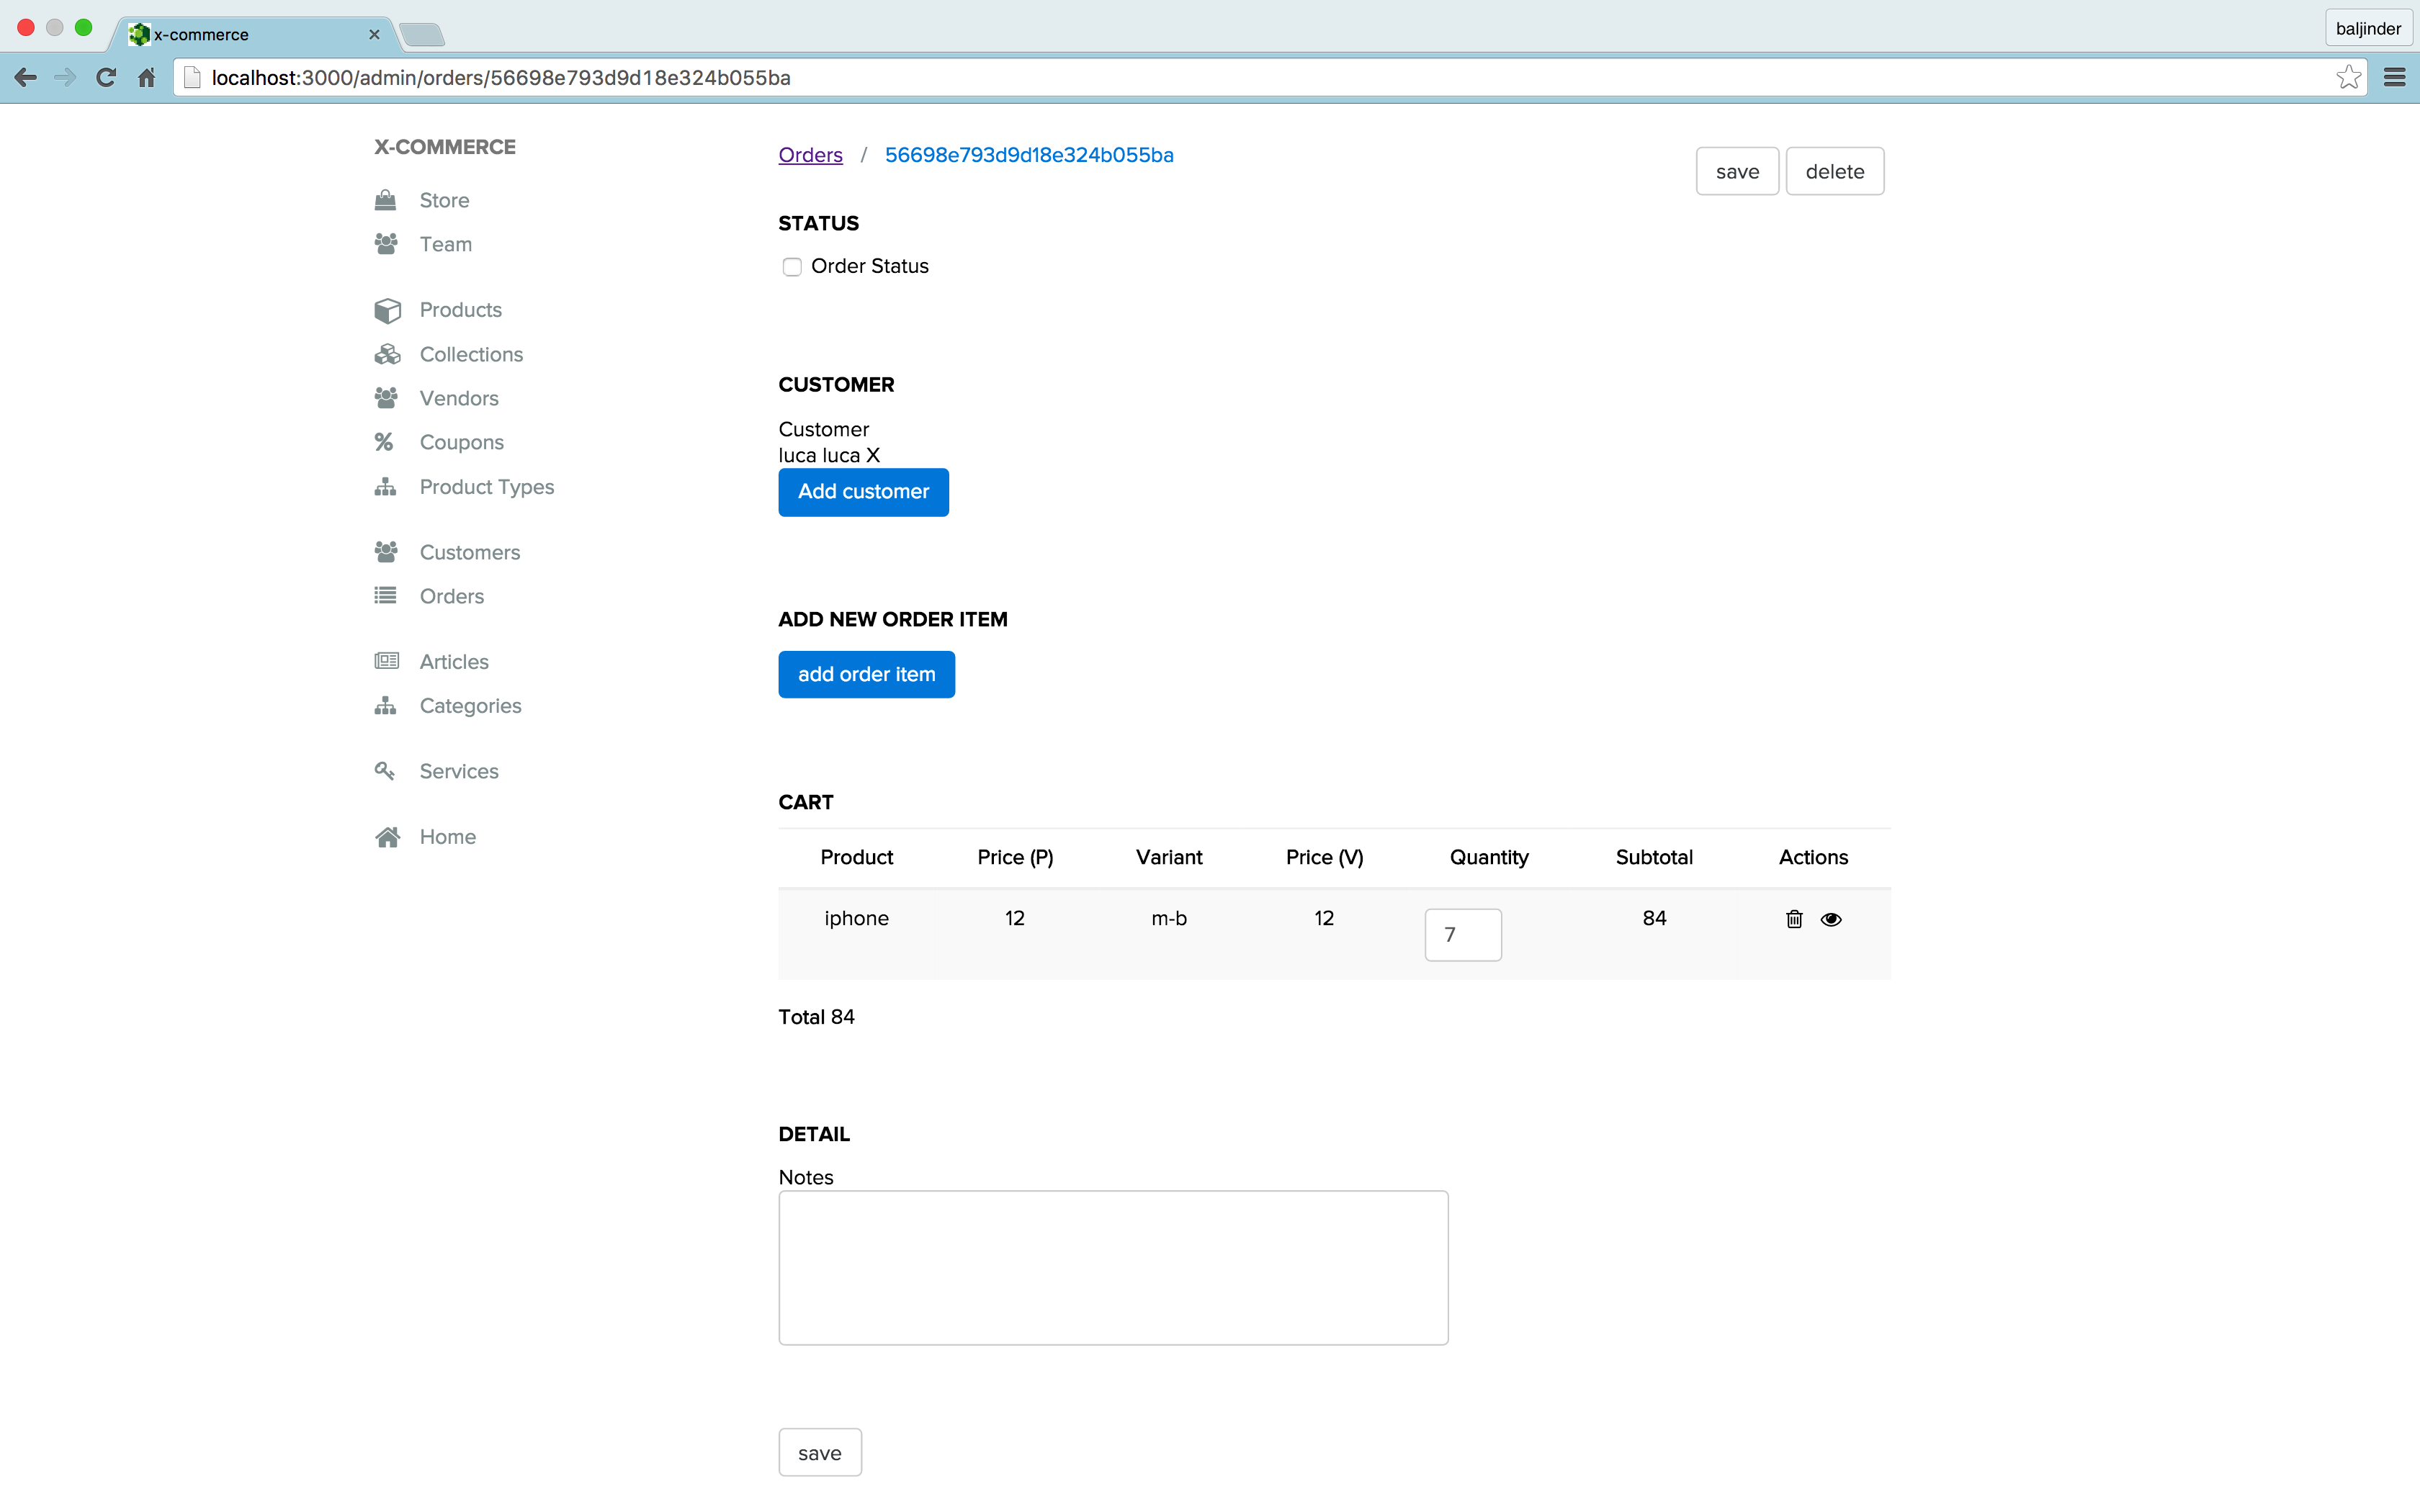
\includegraphics[width=1.0\linewidth]{images/chapter4/page-order-all.png}\hfill
\caption[page order admin-side]{Page order admin-side}
\label{fig:page_order_admin}
\end{figure}
\newpage
% Following shows the vendor page on the admin-side:
\begin{figure}[htb]
\centering
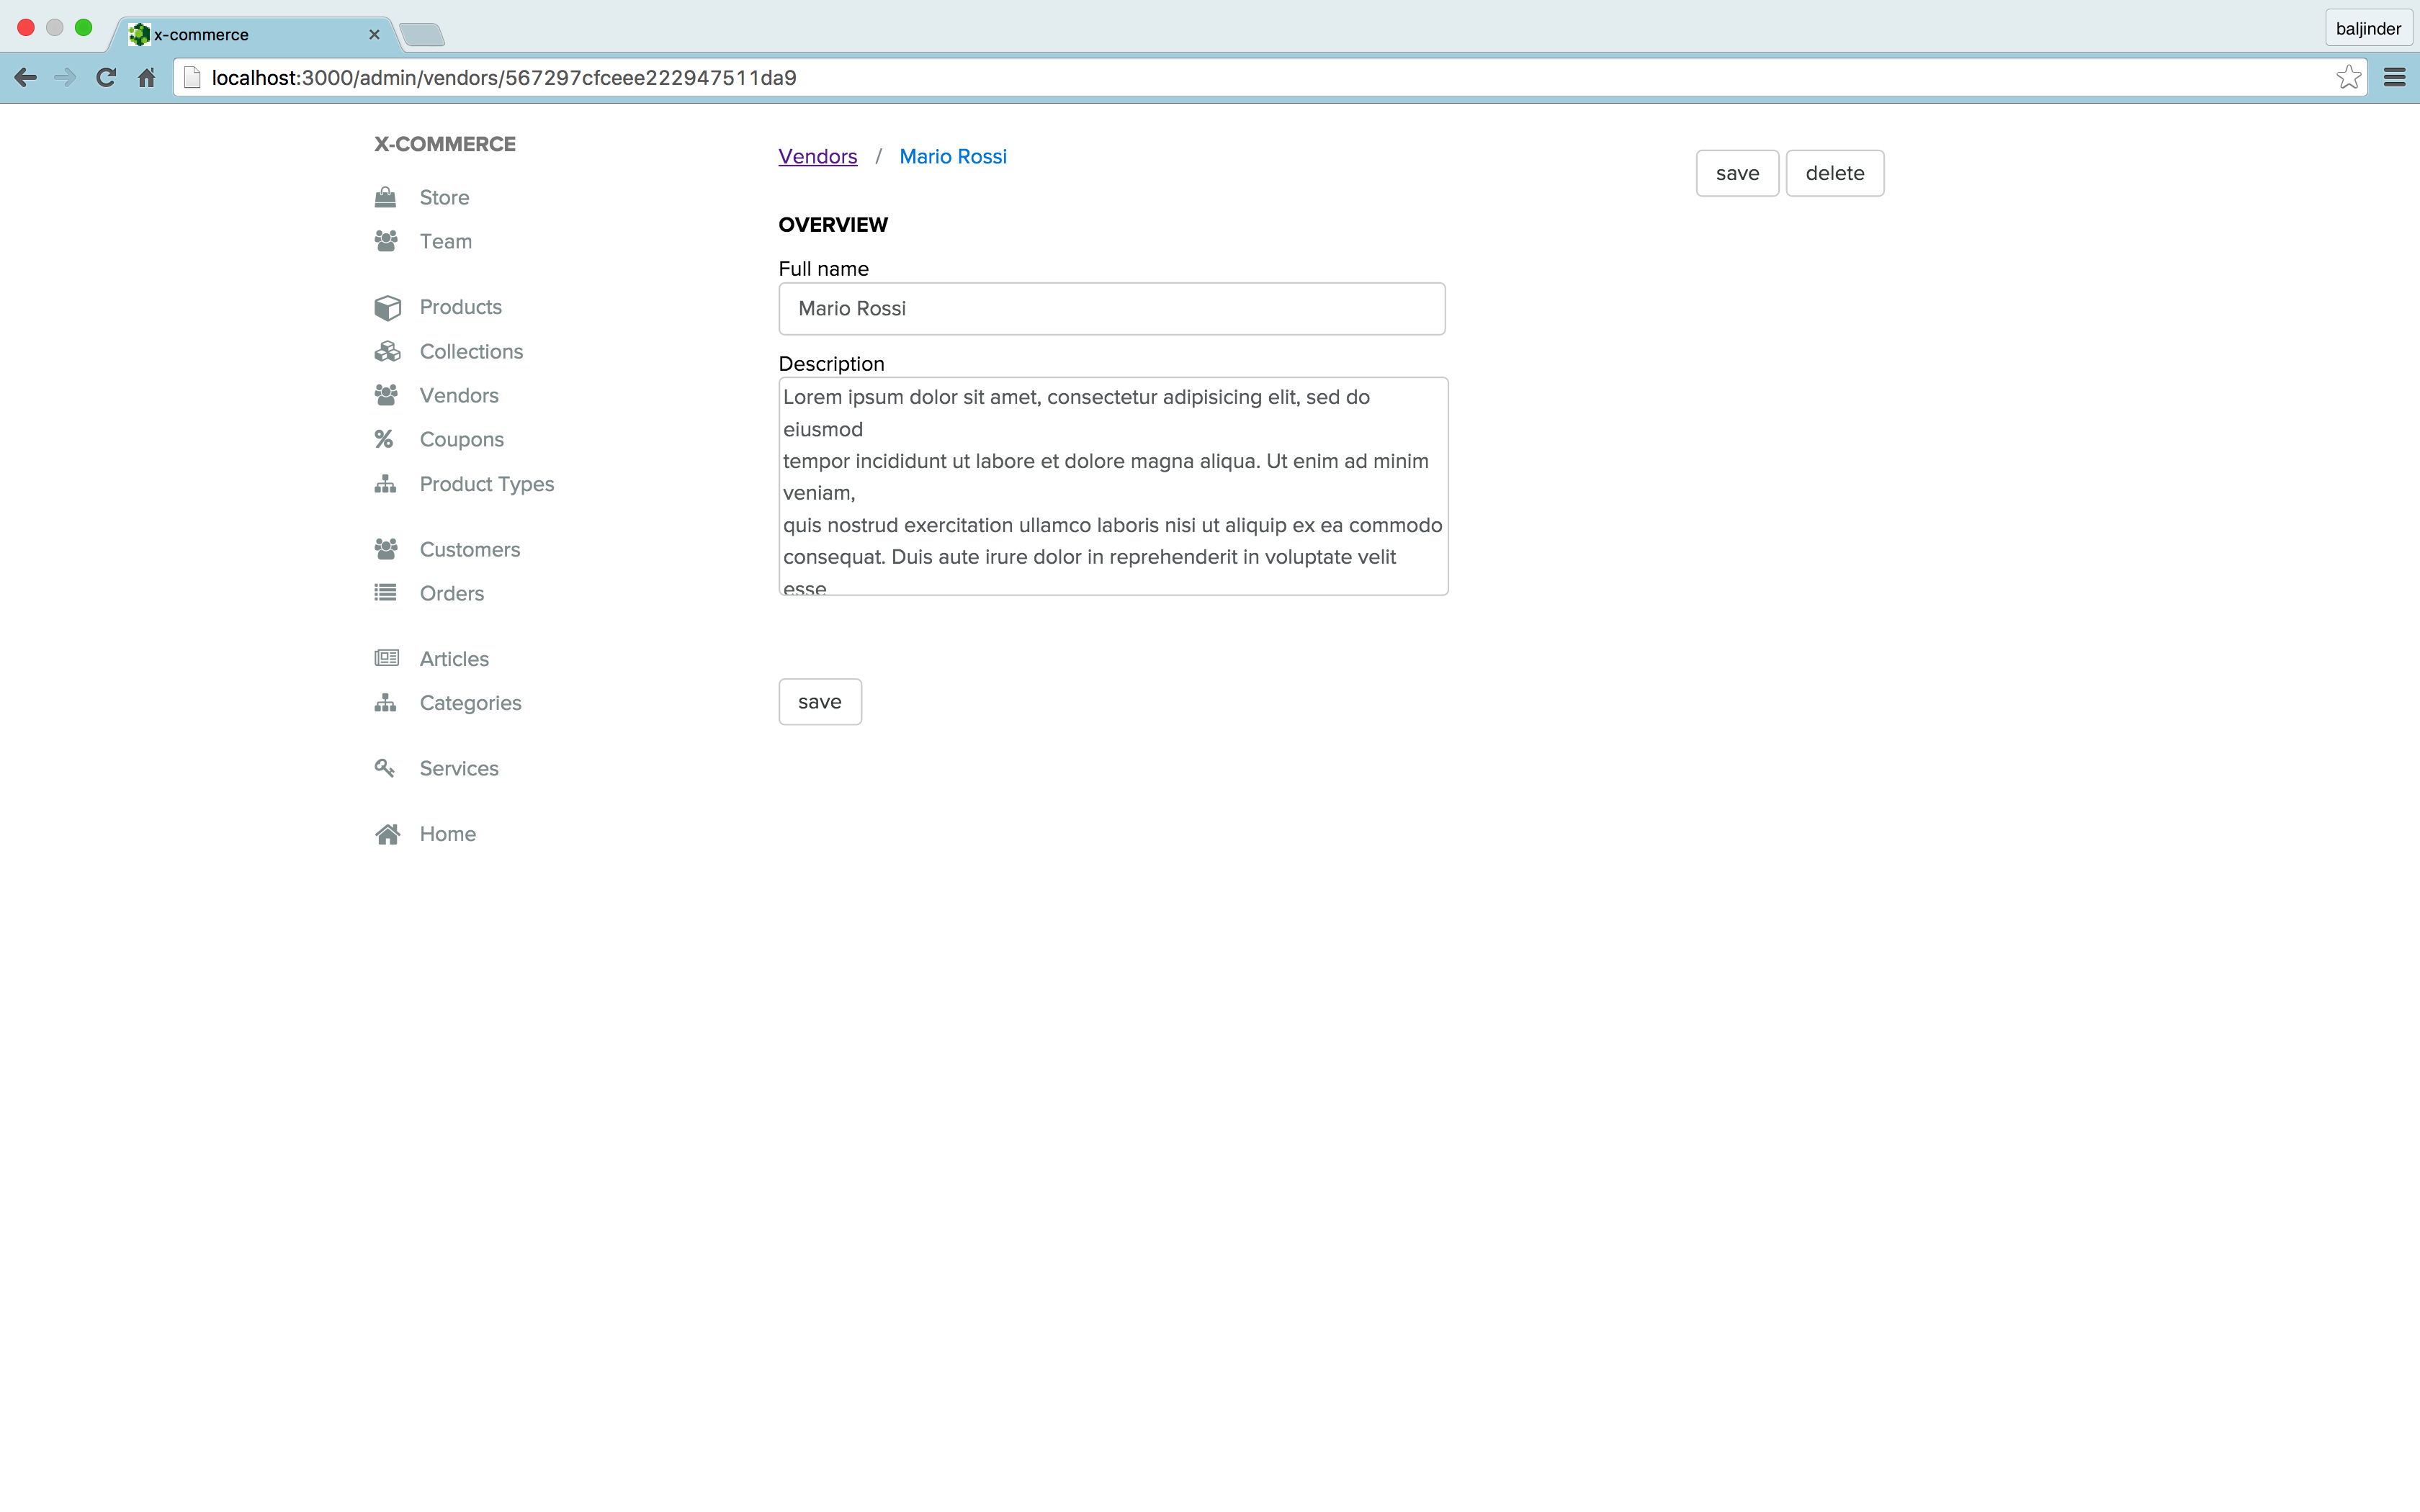
\includegraphics[width=0.84\linewidth]{images/chapter4/page-vendor-all.png}\hfill
\caption[Vendor page on the  admin-side]{Vendor page on the admin-side}
\label{fig:page_vendor_admin}
\end{figure}
% Following shows the coupon page on the admin-side:
\begin{figure}[htb]
\centering
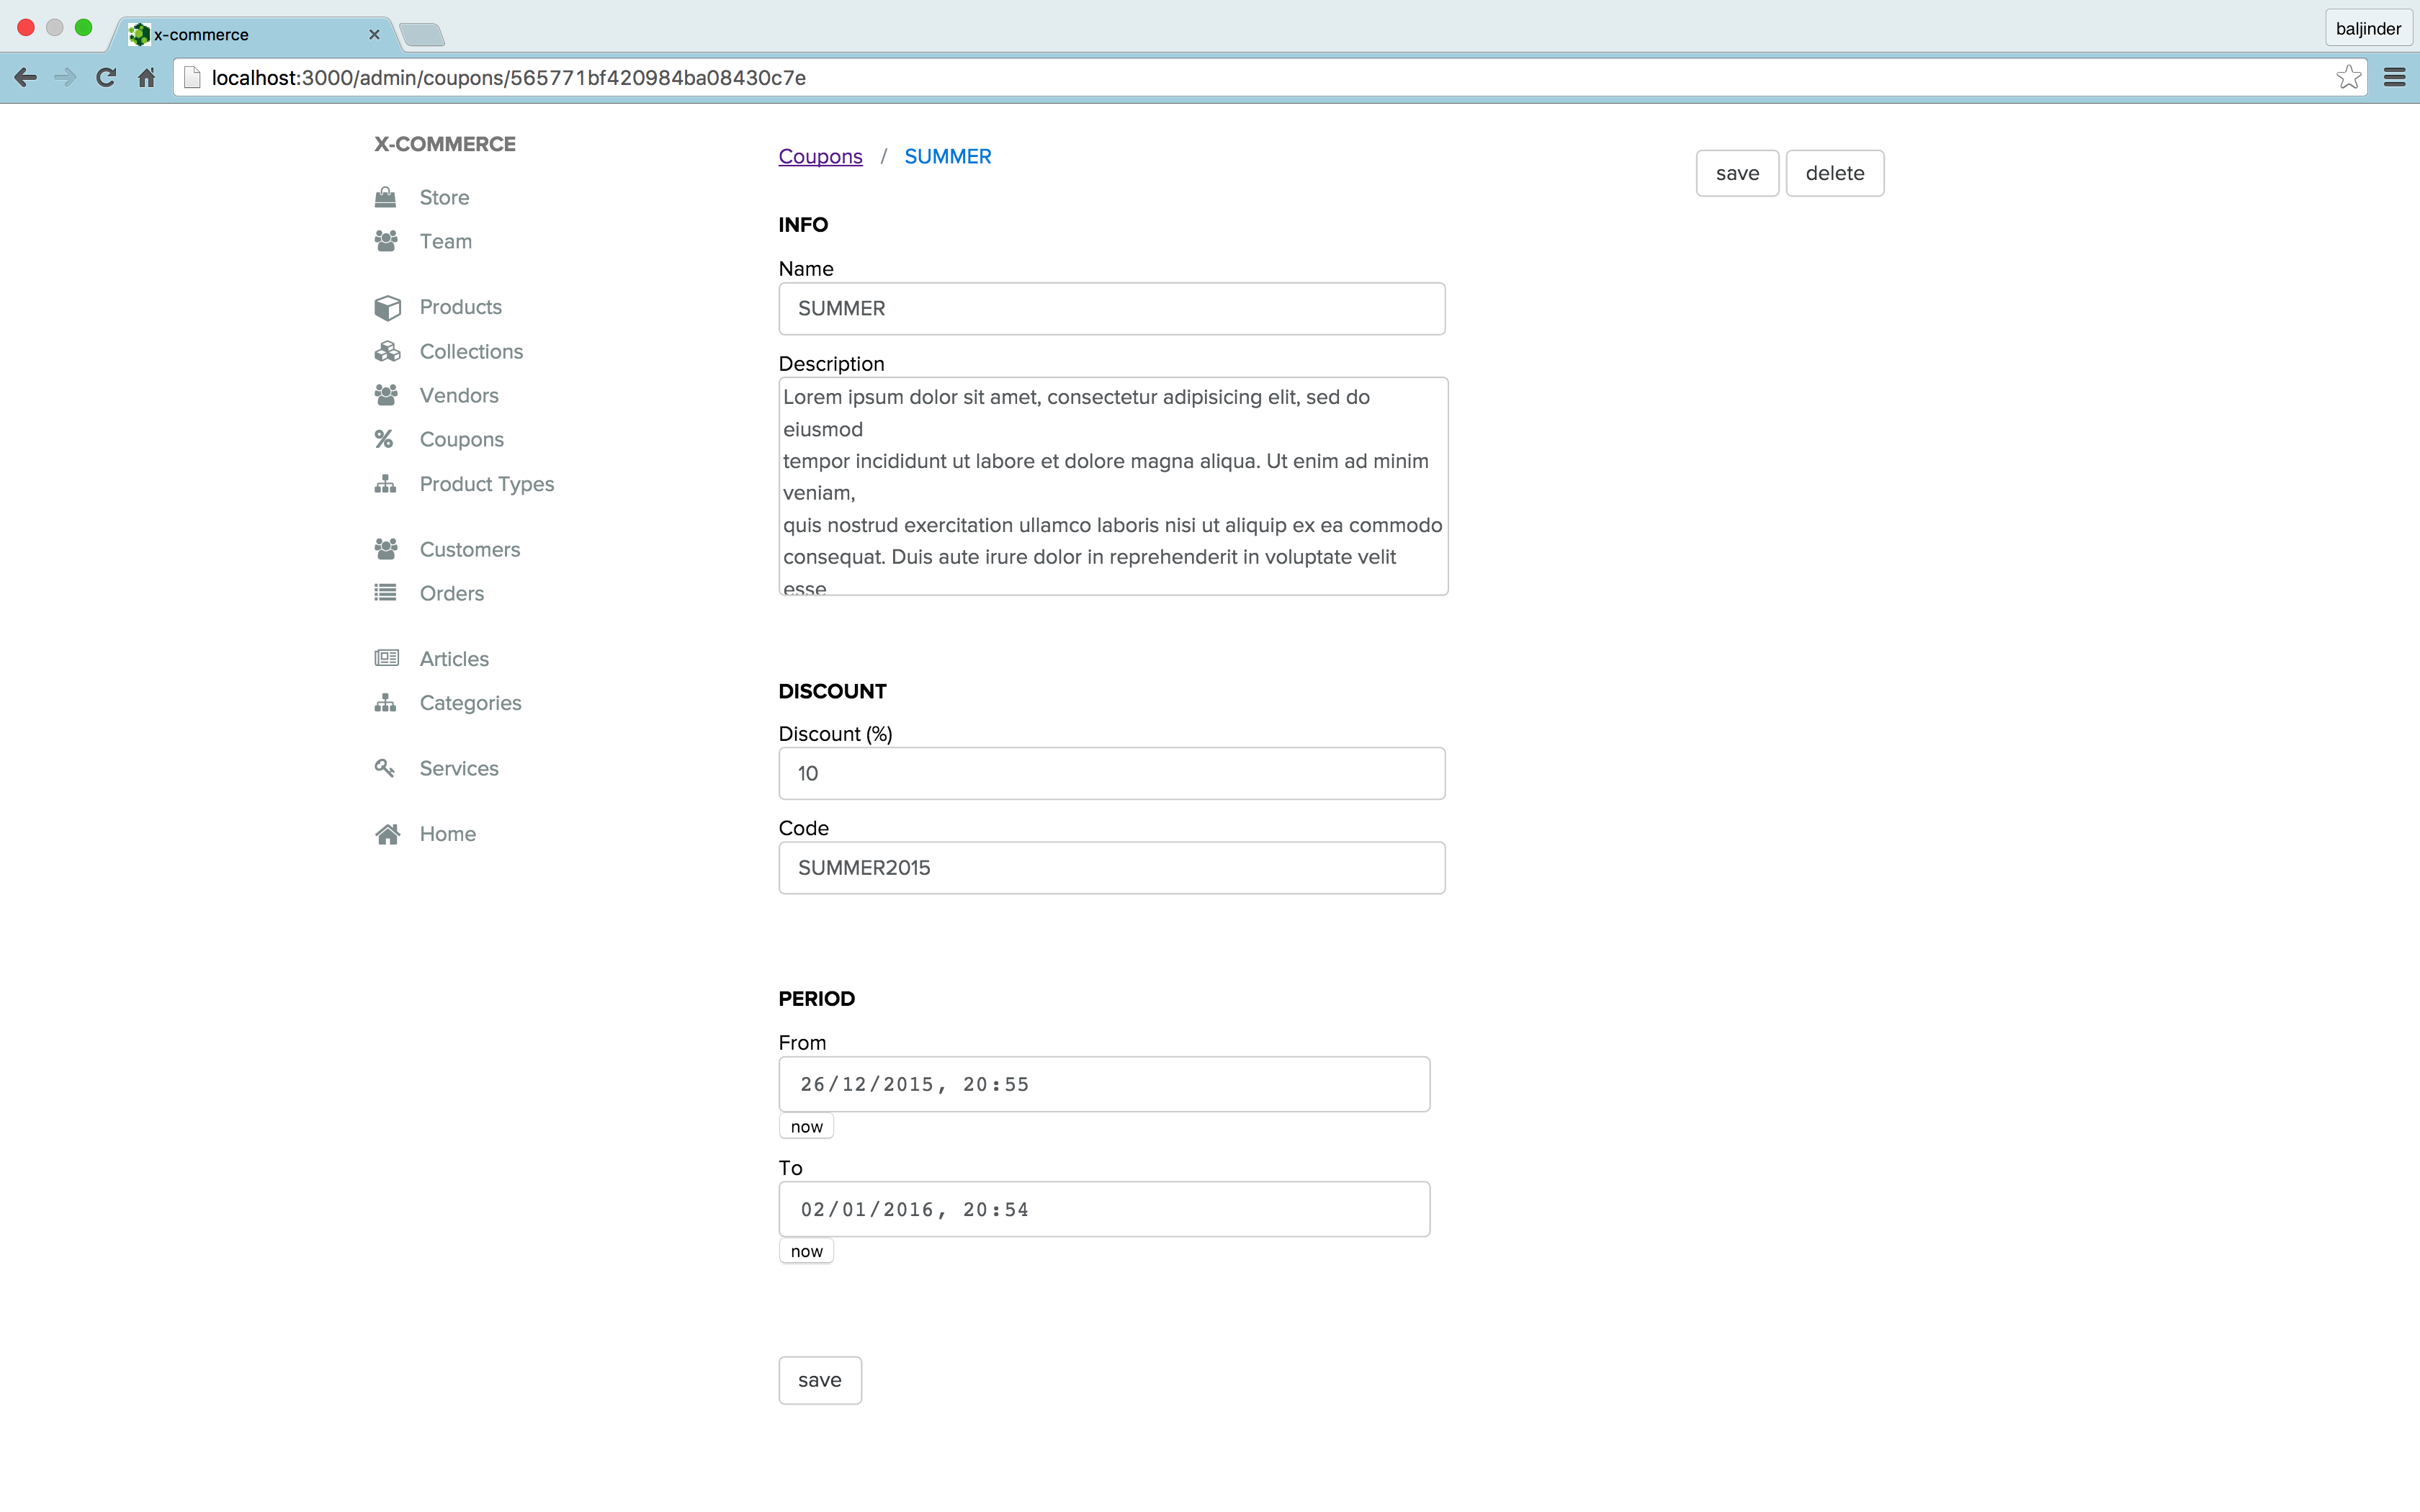
\includegraphics[width=0.84\linewidth]{images/chapter4/page-coupon-all.png}\hfill
\caption[Coupon page on the admin-side]{Coupon page on the admin-side}
\label{fig:page_coupon_admin}
\end{figure}
% Following shows the products page on the admin-side:
\newpage
\begin{figure}[htb]
\centering
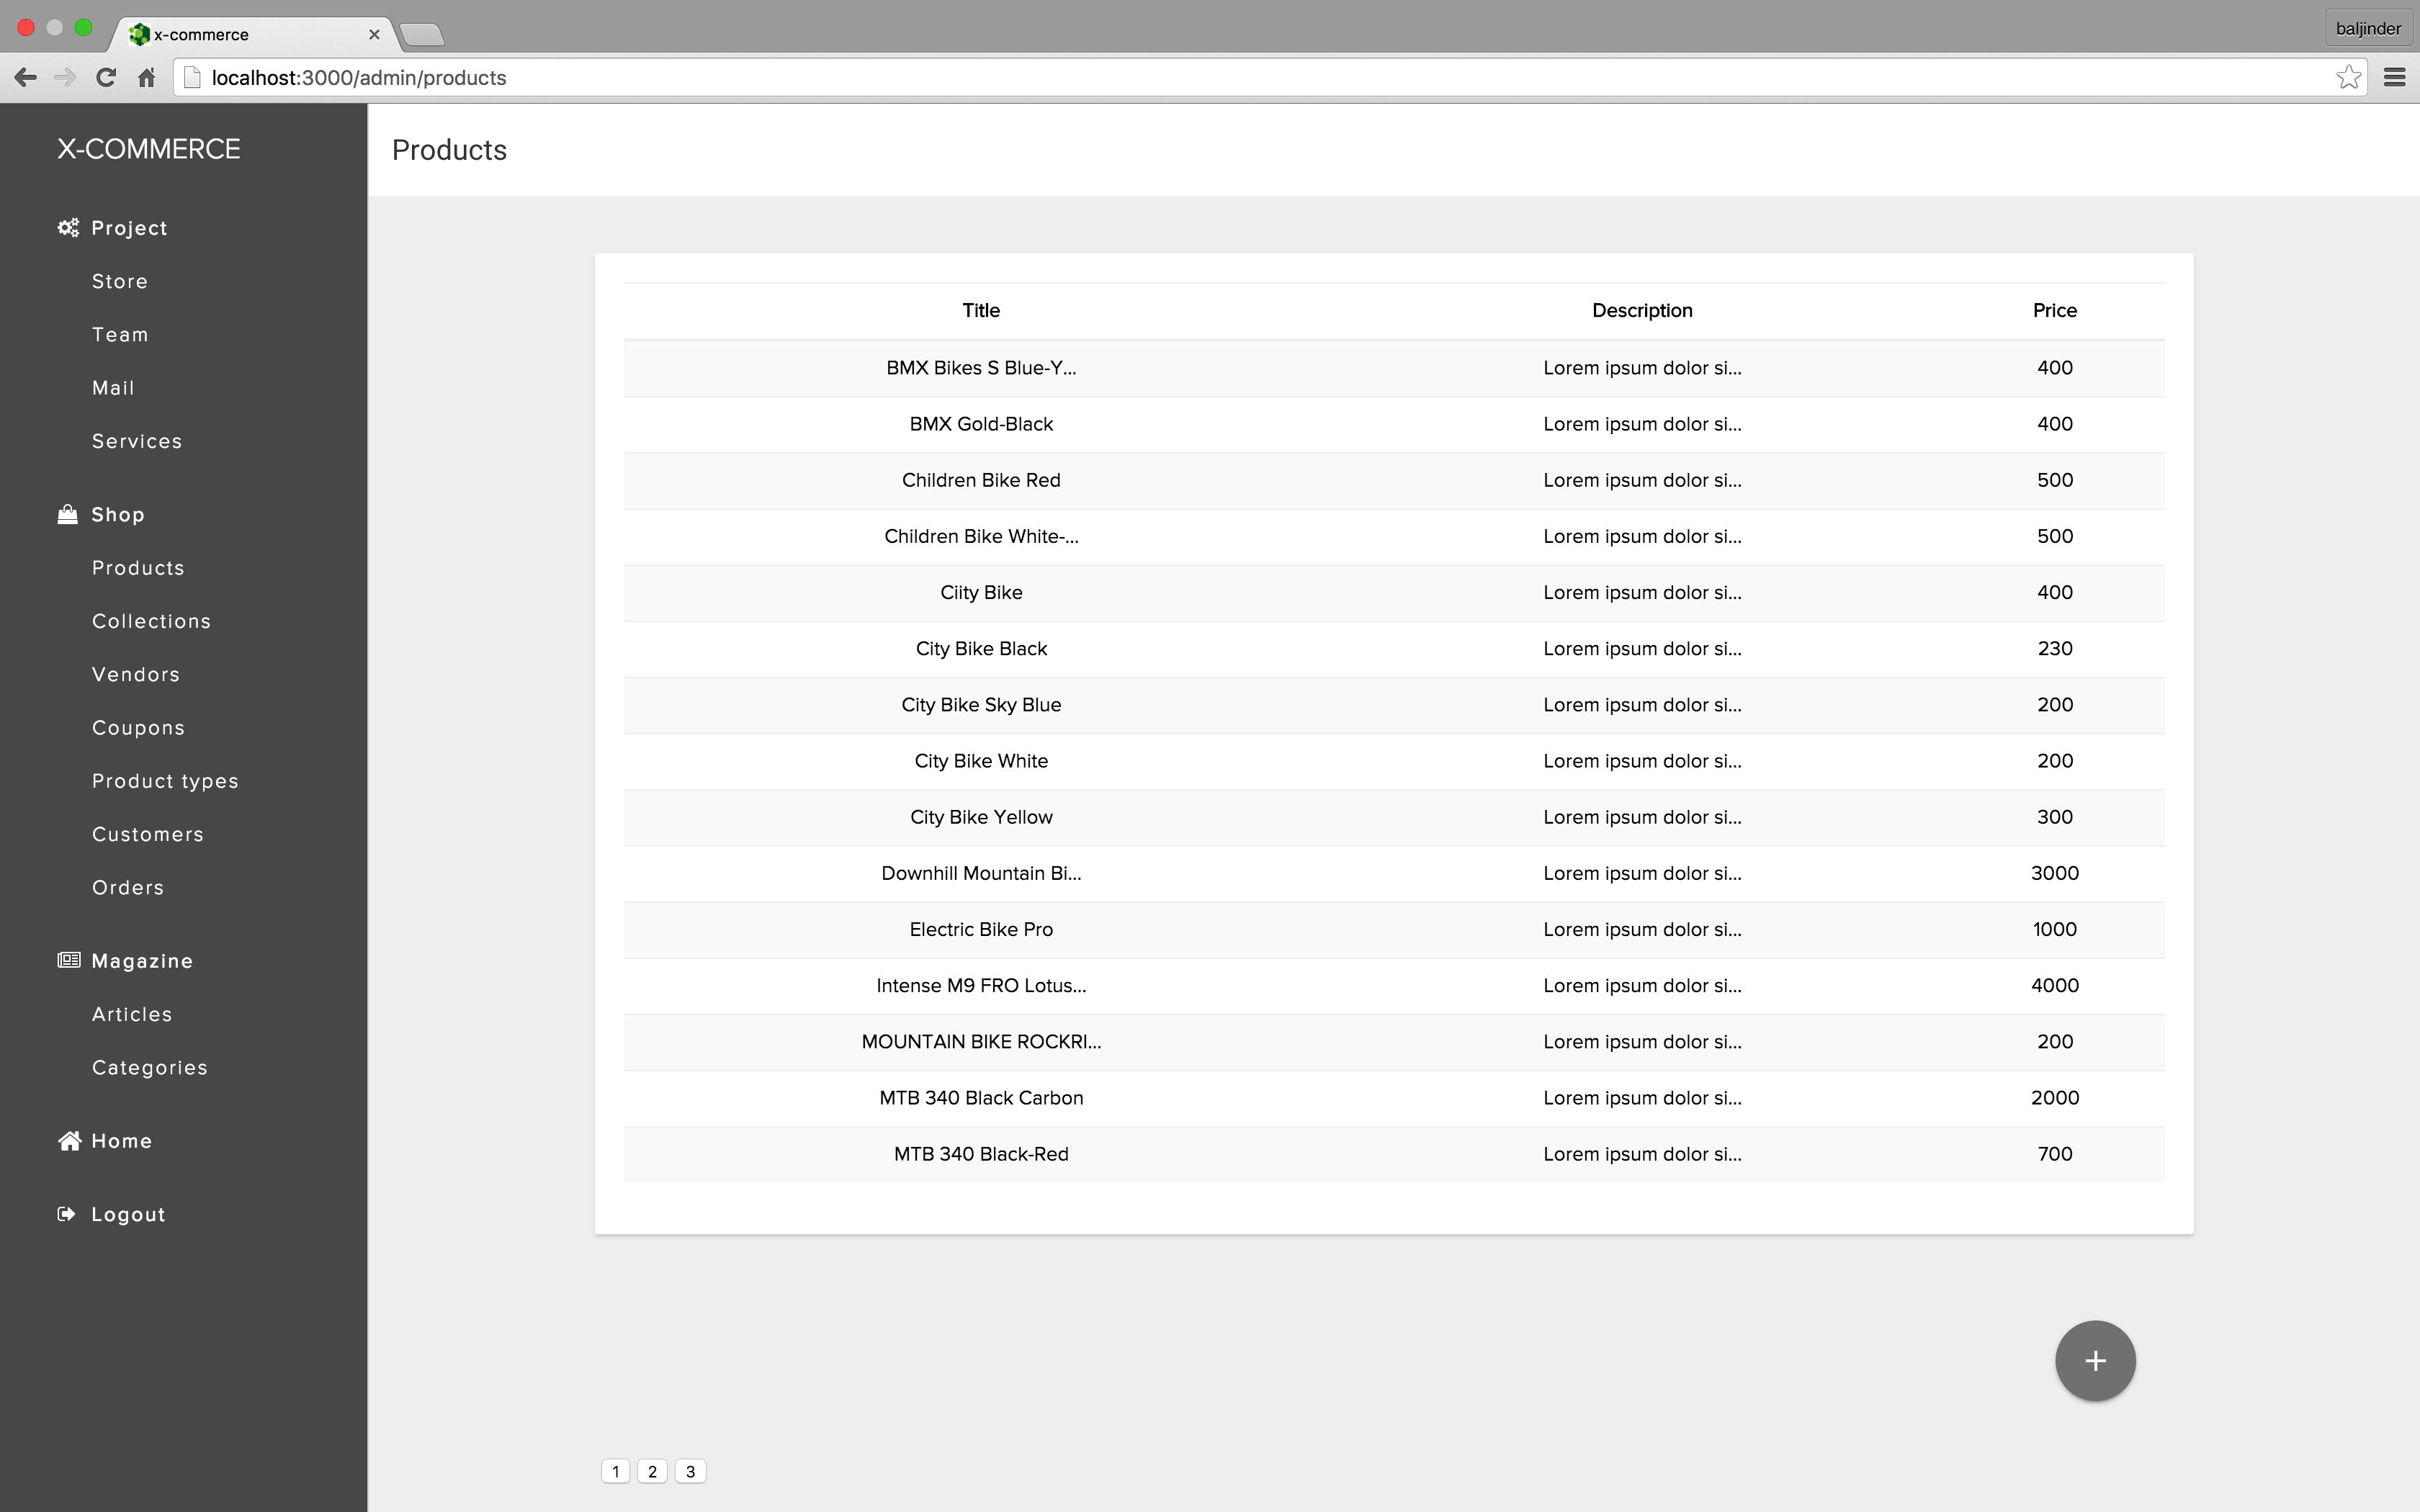
\includegraphics[width=0.84\linewidth]{images/chapter4/page-products-all.png}\hfill
\caption[Products page on the admin-side]{Products page on the admin-side}
\label{fig:page_products_admin}
\end{figure}
% Following shows the products page  on the client-side:
\begin{figure}[htb]
\centering
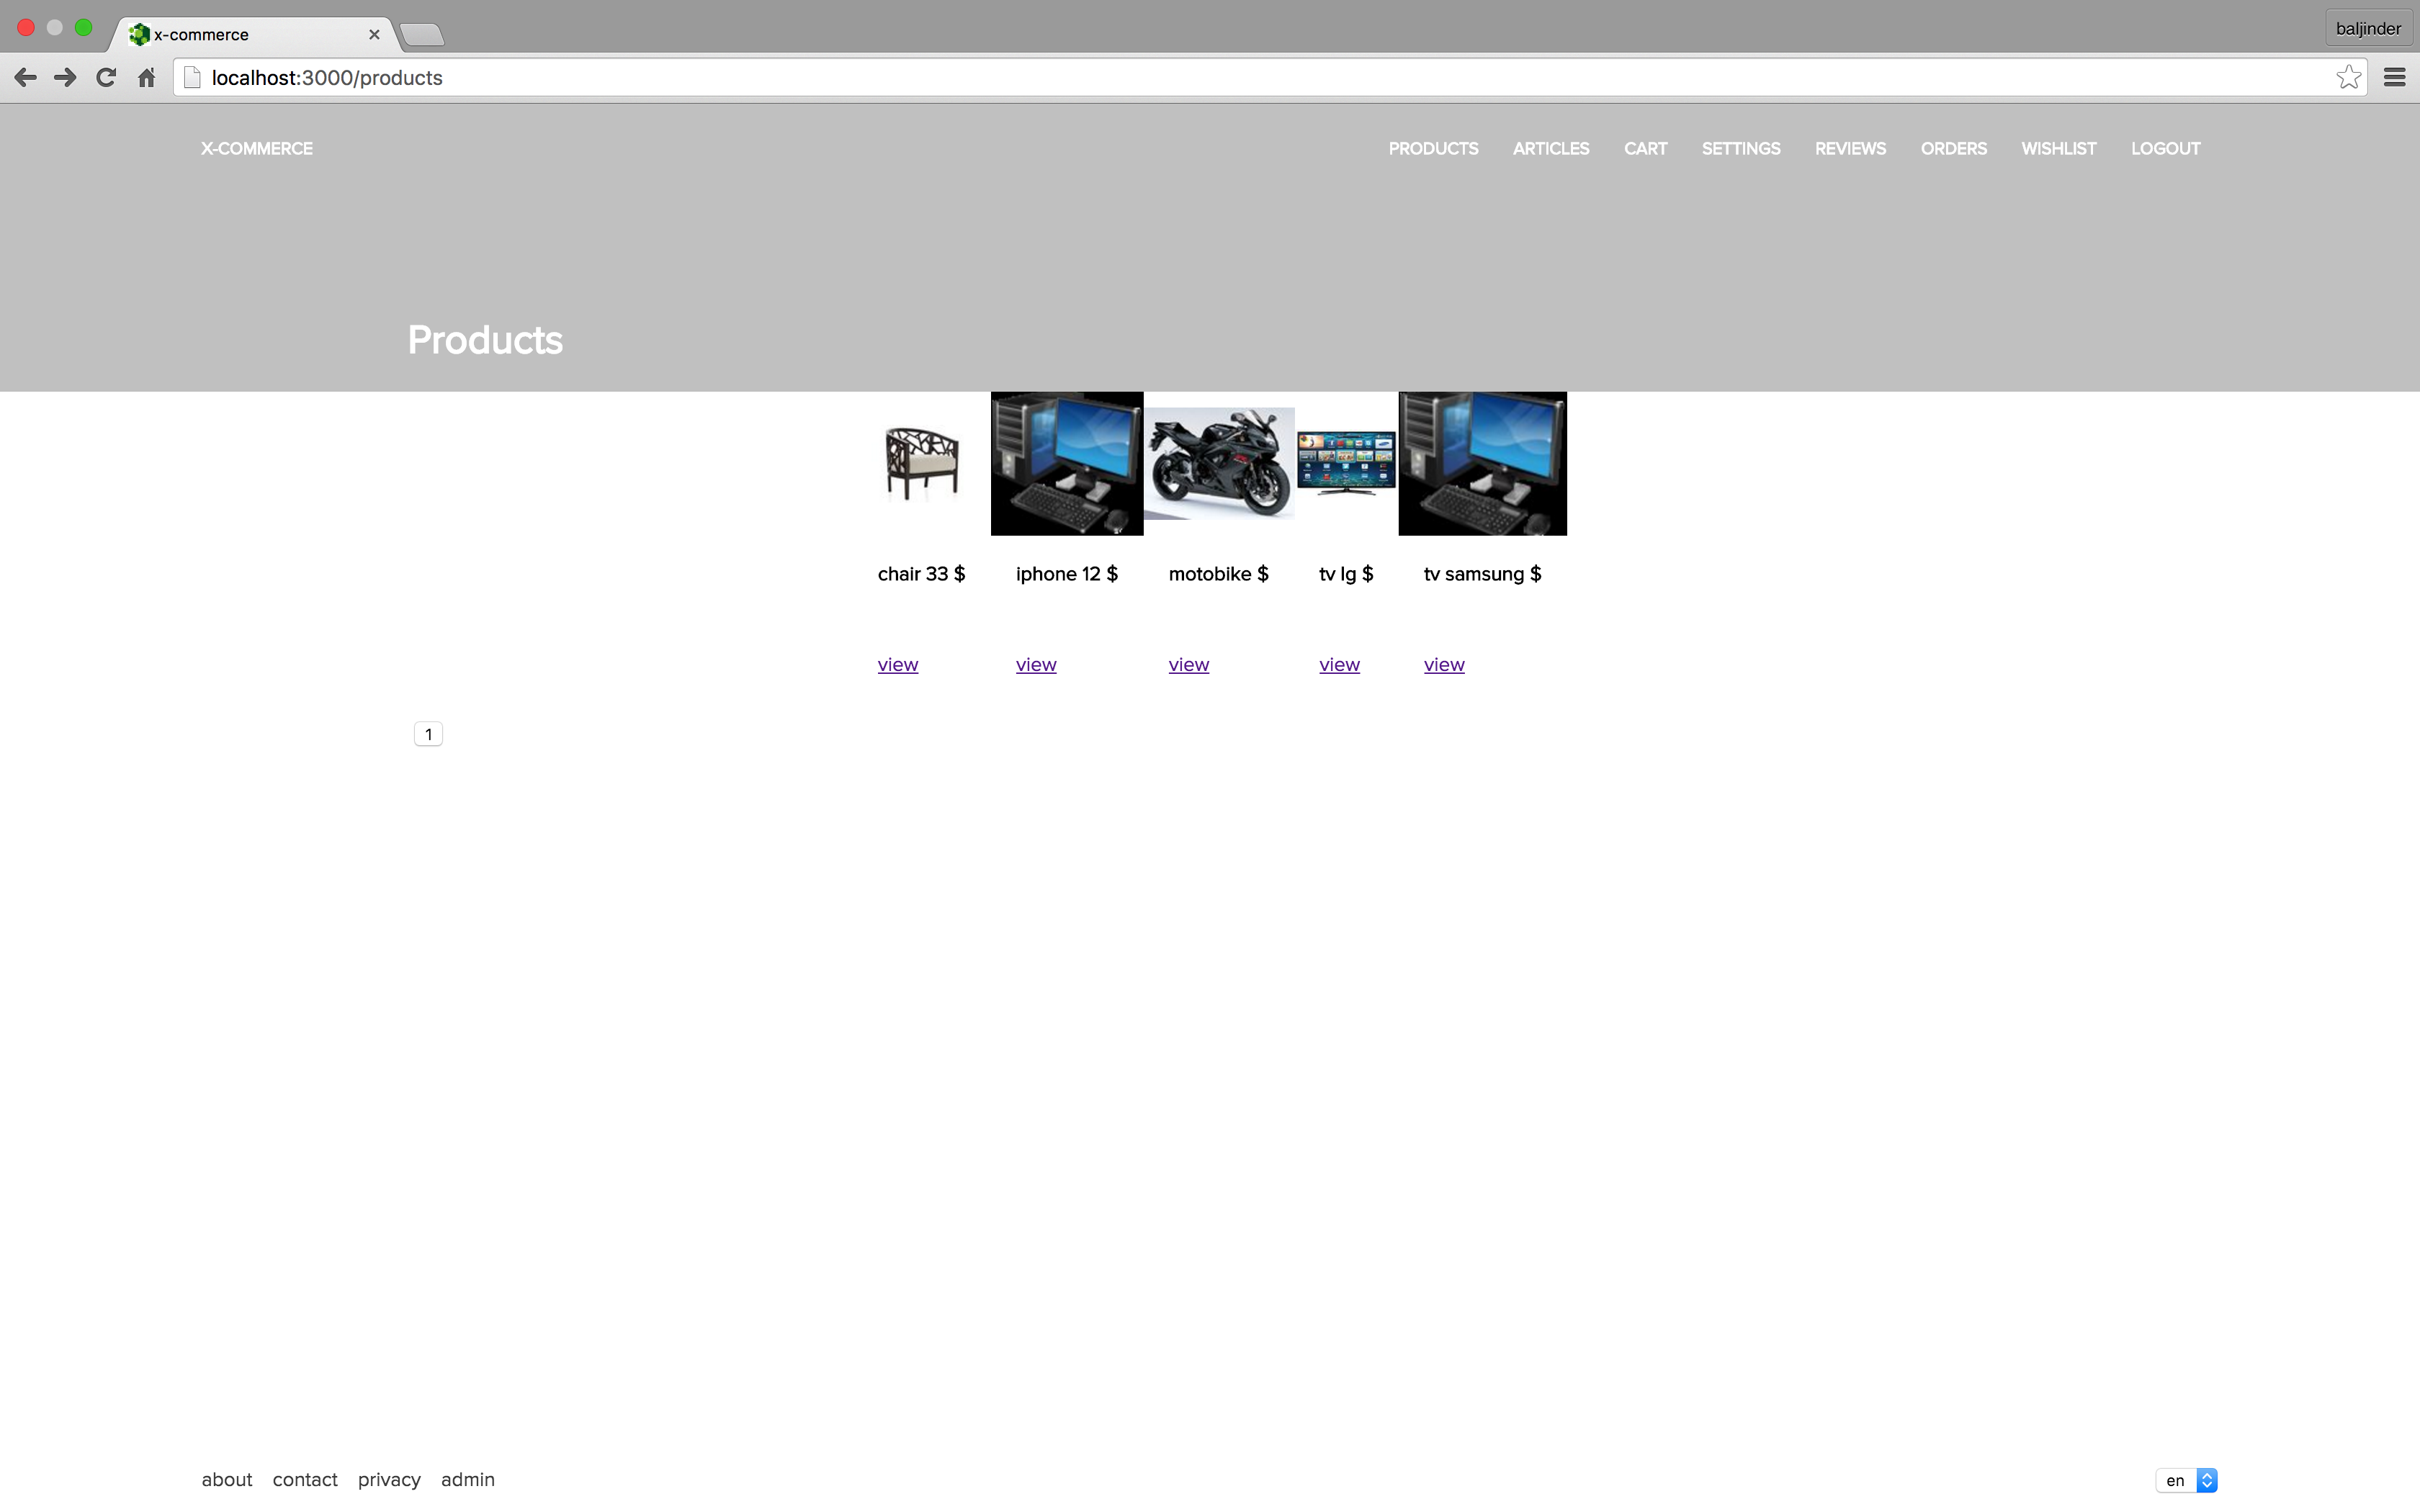
\includegraphics[width=0.84\linewidth]{images/chapter4/page-products-all-cli.png}\hfill
\caption[Products page on the client-side]{Products page on the client-side}
\label{fig:page_products_cli}
\end{figure}
\newpage
% Following shows the variants page on the admin-side:
\begin{figure}[htb]
\centering
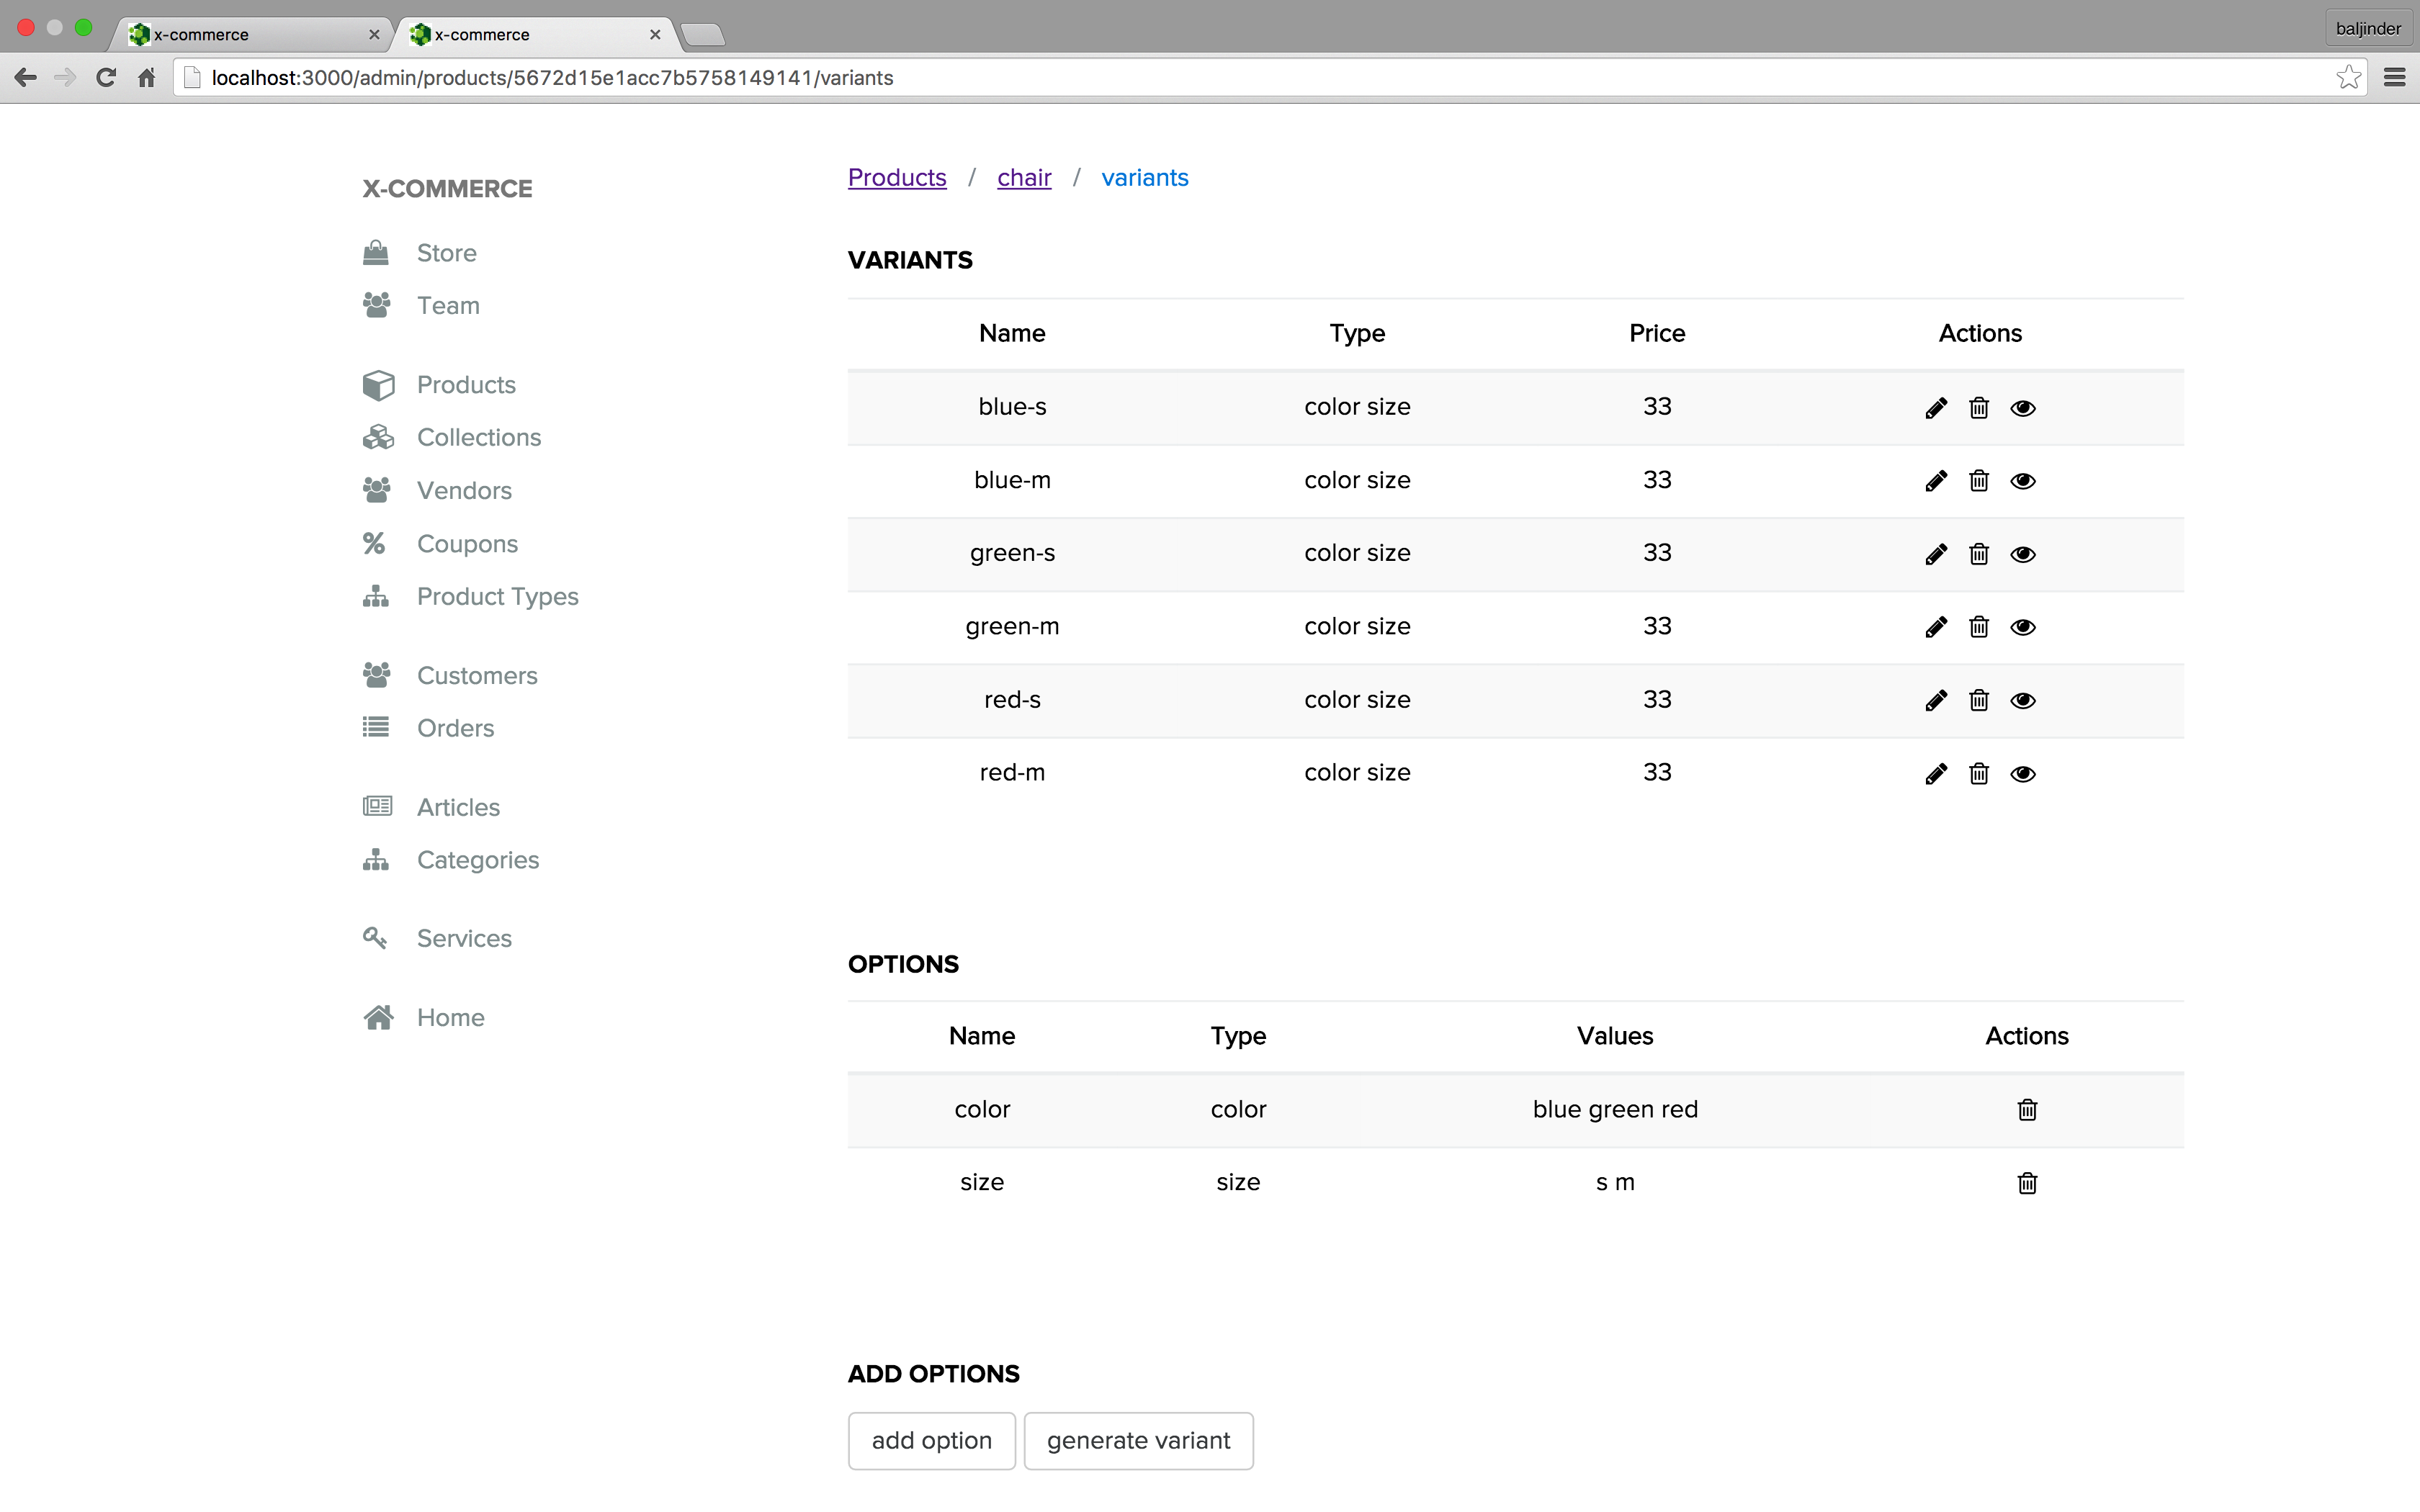
\includegraphics[width=0.84\linewidth]{images/chapter4/page-variants.png}\hfill
\caption[Variants page on the admin-side]{Variants page on the admin-side}
\label{fig:page_variants_admin}
\end{figure}
% Following shows the collection page on the client-side:
\begin{figure}[htb]
\centering
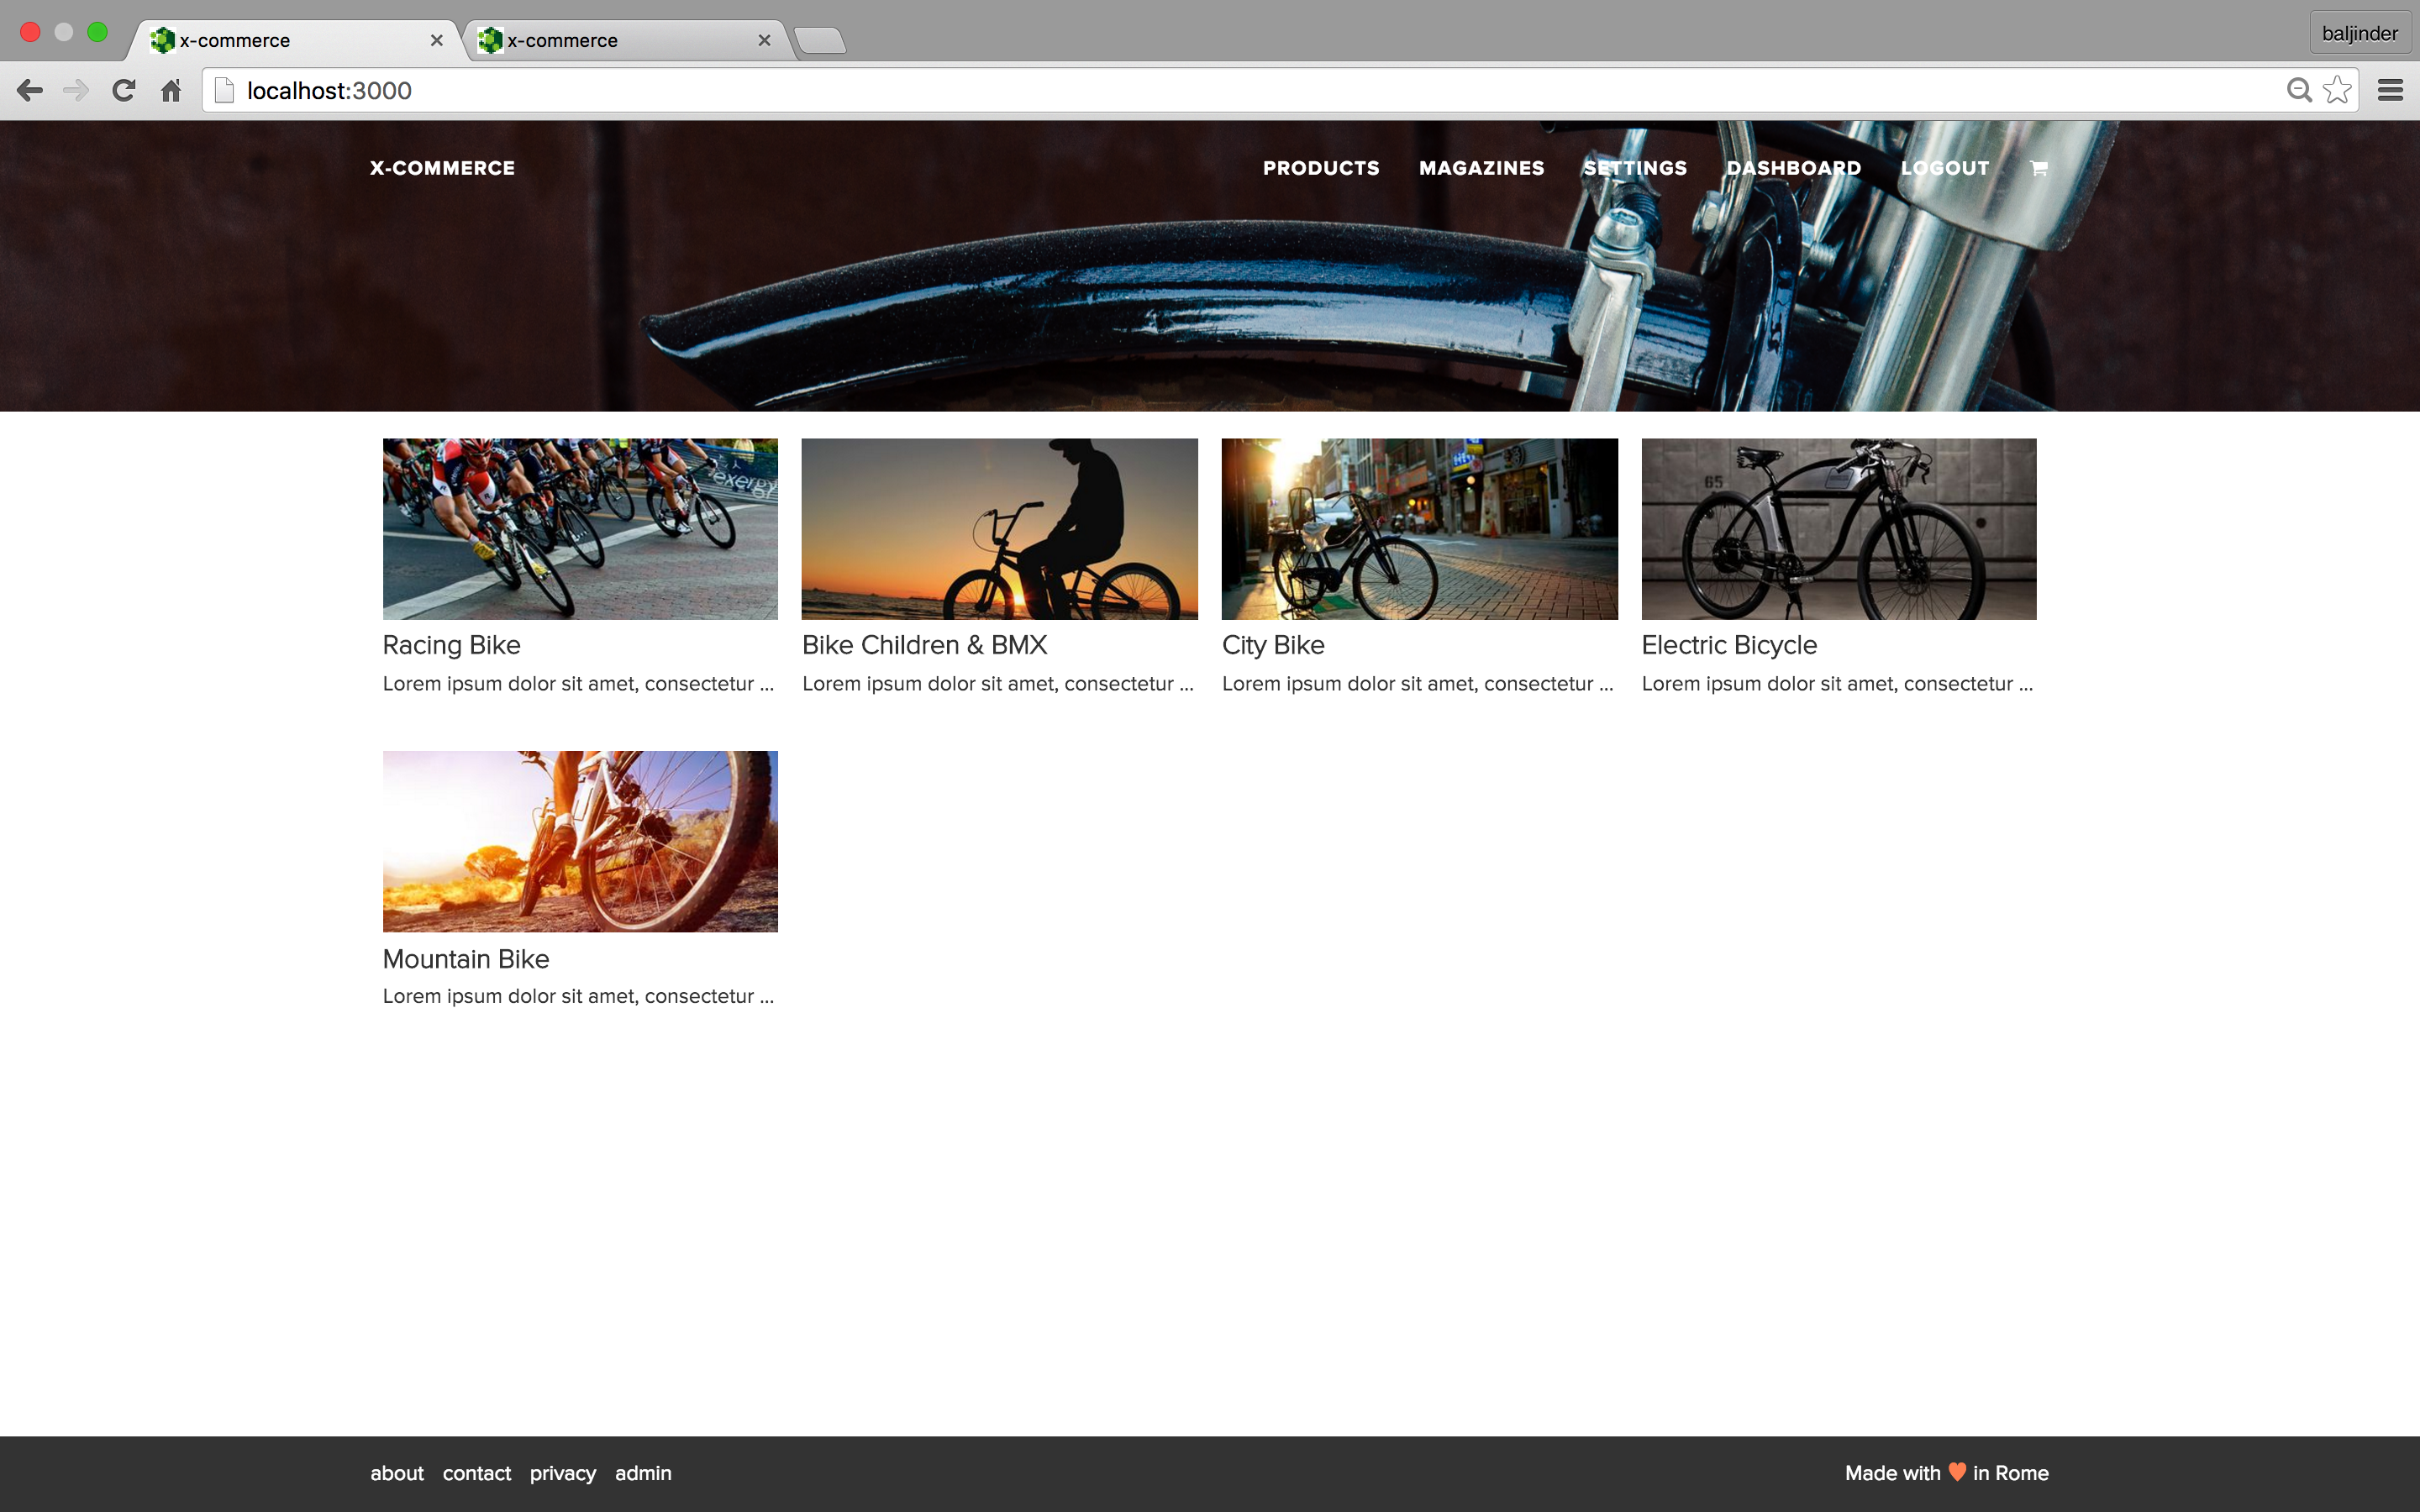
\includegraphics[width=0.84\linewidth]{images/chapter4/page-collection.png}\hfill
\caption[Collection page on the client-side]{Collection page on the client-side}
\label{fig:page_collection_cli}
\end{figure}
\newpage
% Following shows the customer page on the admin-side:
\begin{figure}[htb]
\centering
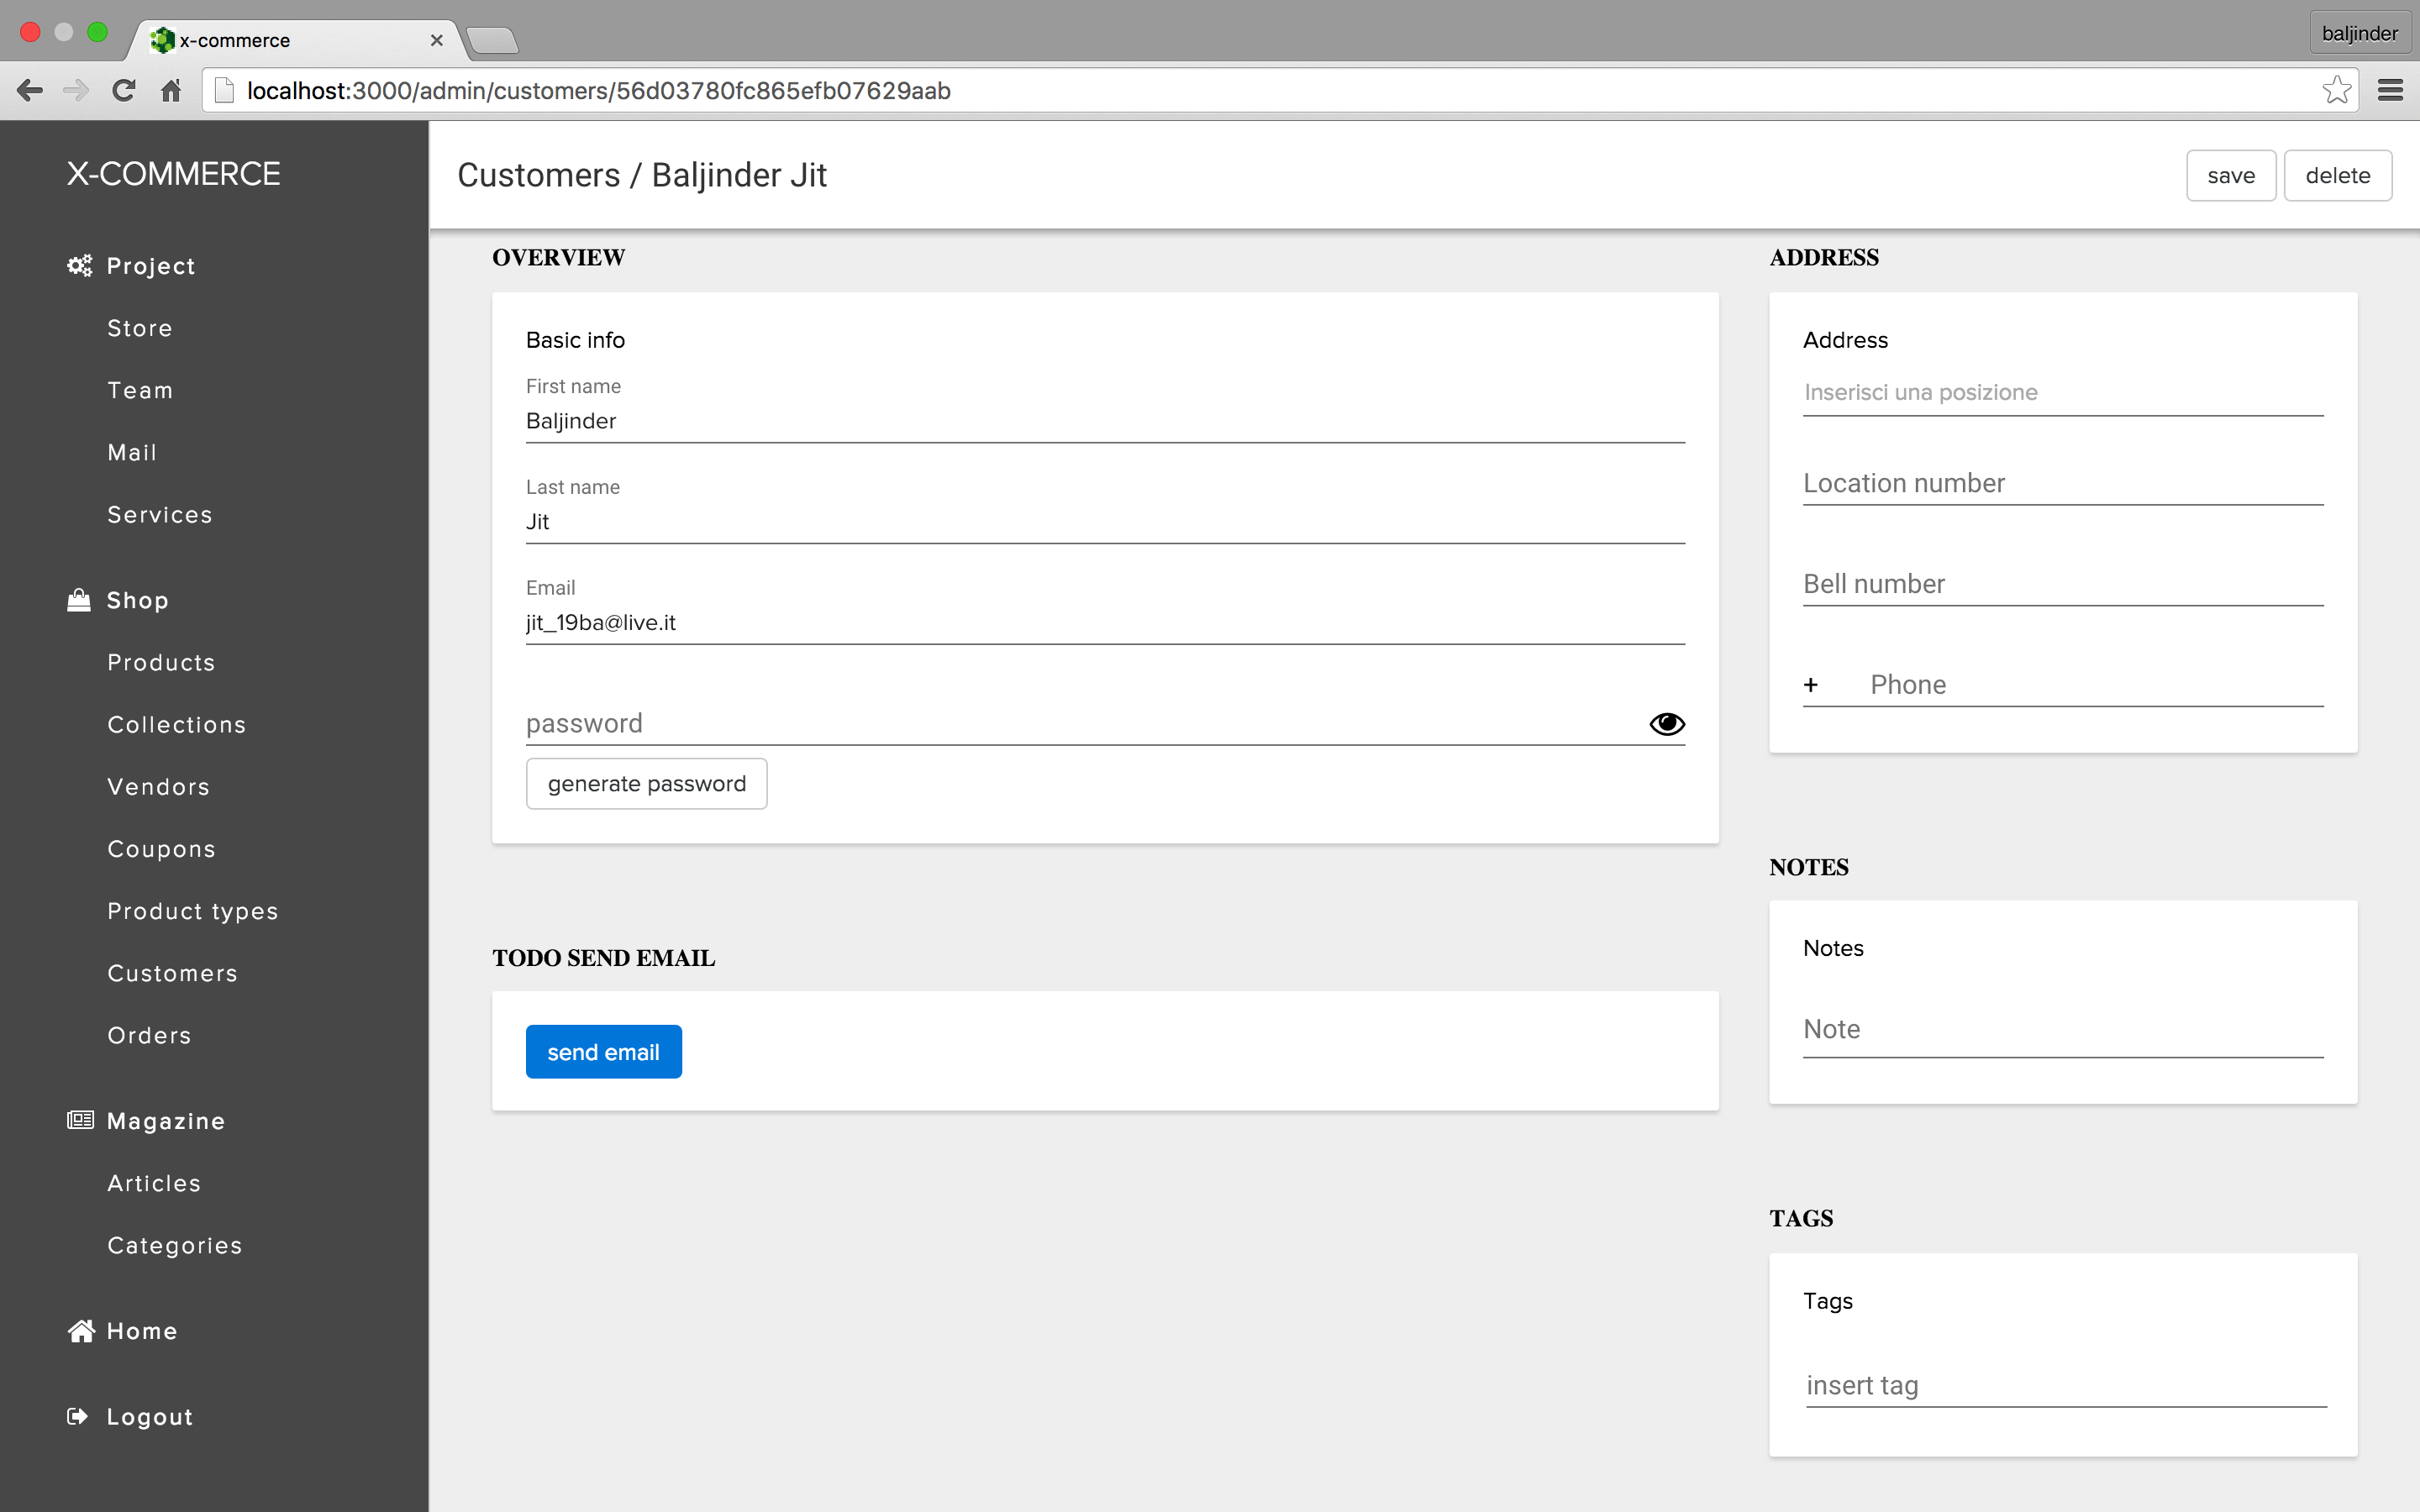
\includegraphics[width=0.84\linewidth]{images/chapter4/page-customer.png}\hfill
\caption[Customer page on the admin-side]{Customer page on the admin-side}
\label{fig:page_customer_admin}
\end{figure}
% Following shows the cart page on the admin-side:
\begin{figure}[htb]
\centering
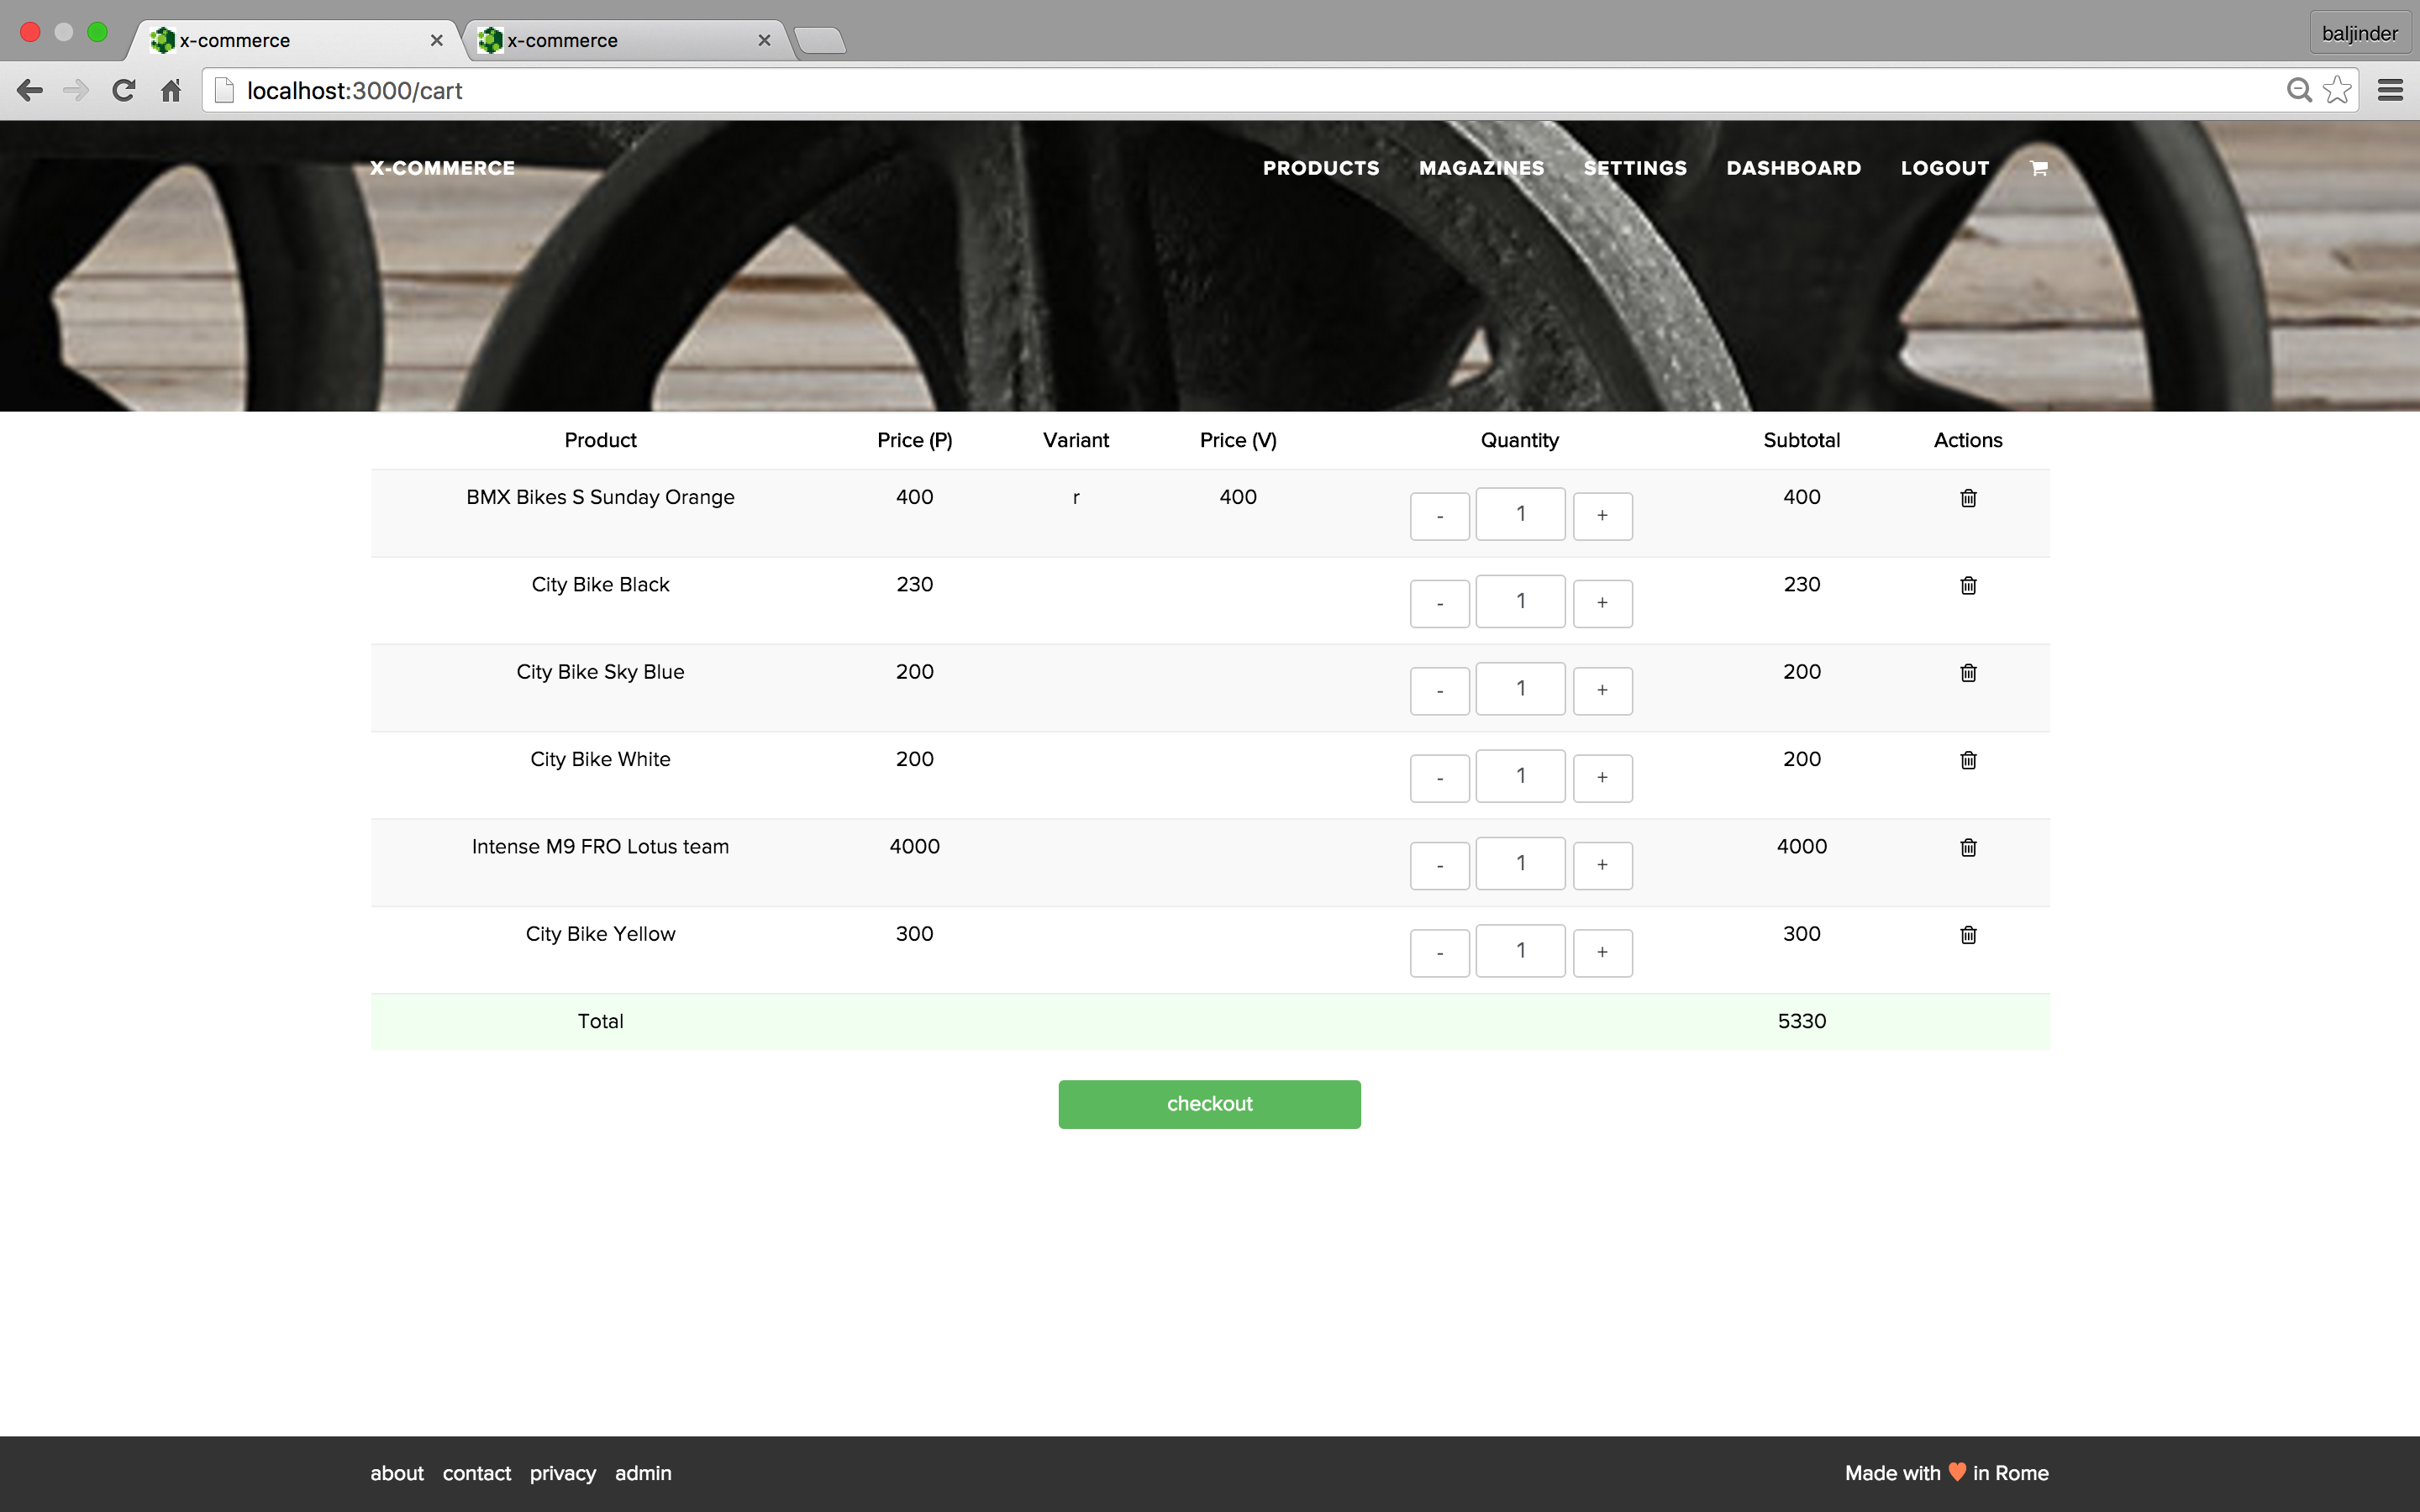
\includegraphics[width=0.84\linewidth]{images/chapter4/page-cart.png}\hfill
\caption[Cart page on the admin-side]{Cart page on the admin-side}
\label{fig:page_cart_cli}
\end{figure}
\newpage
% Following shows the article page on the admin-side:
\begin{figure}[htb]
\centering
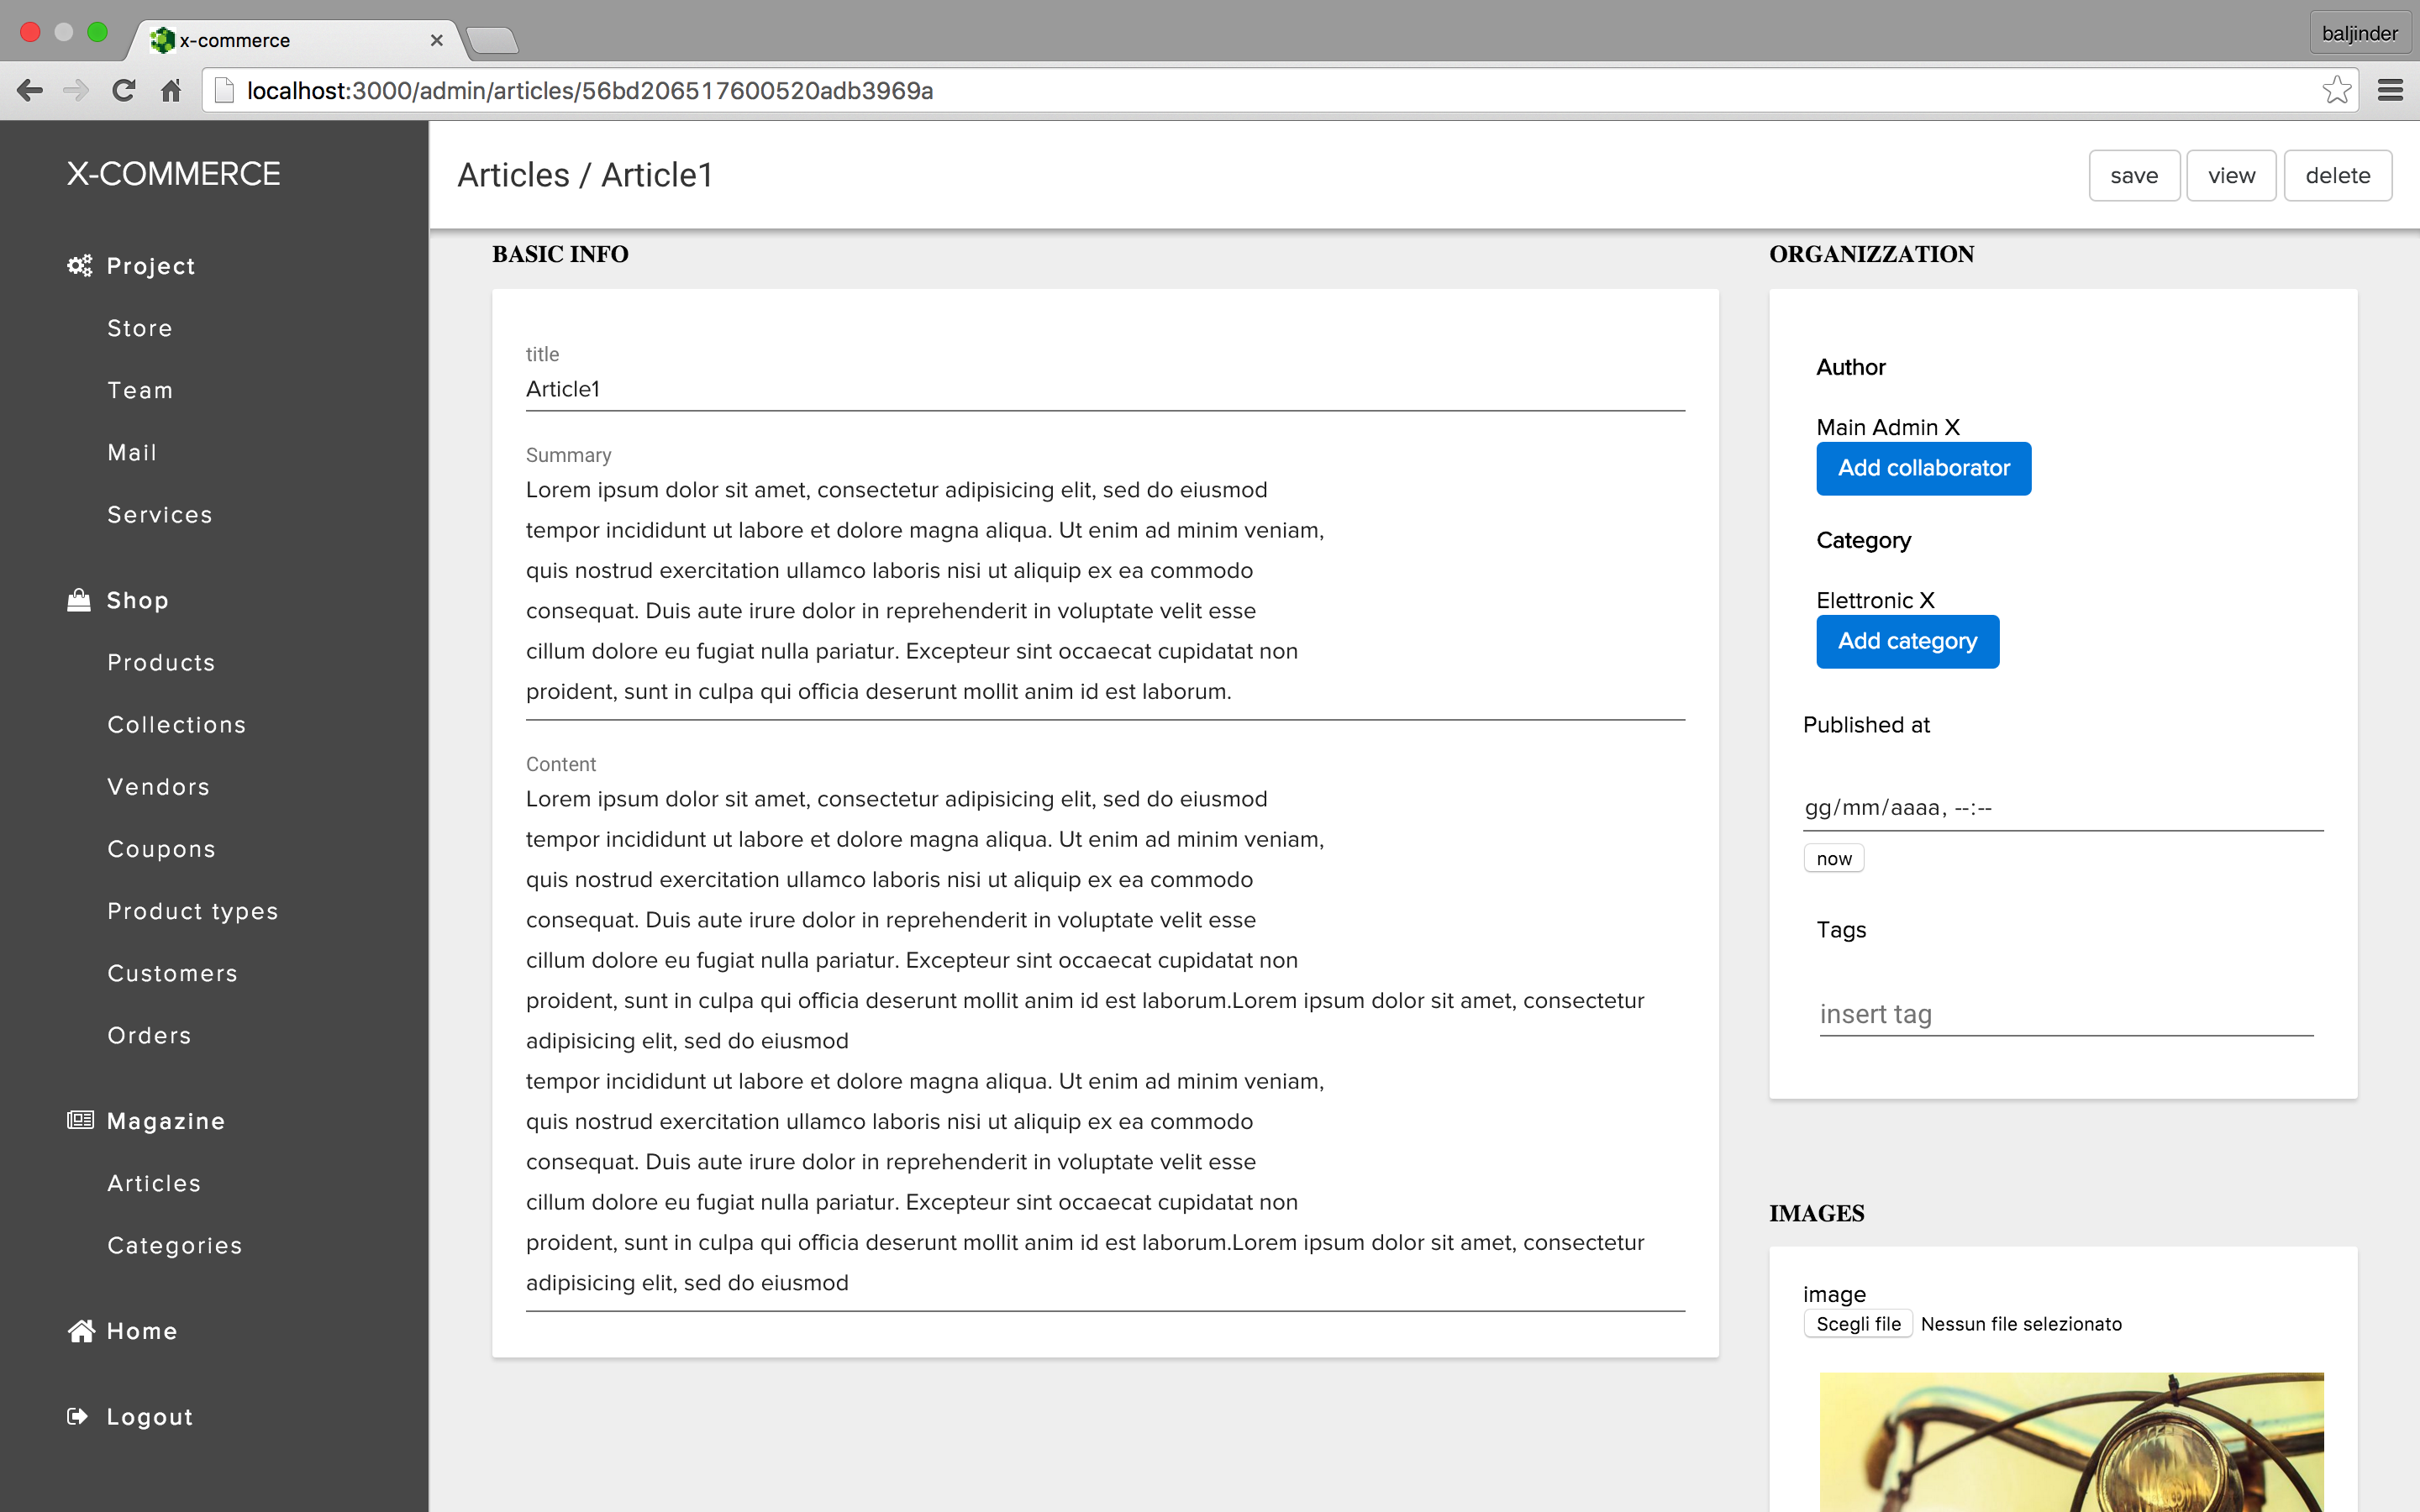
\includegraphics[width=0.84\linewidth]{images/chapter4/page-article-adm.png}\hfill
\caption[Article page on the admin-side]{Article page on the admin-side}
\label{fig:page_article_admin}
\end{figure}
% Following shows the article page on the client-side:
\begin{figure}[htb]
\centering
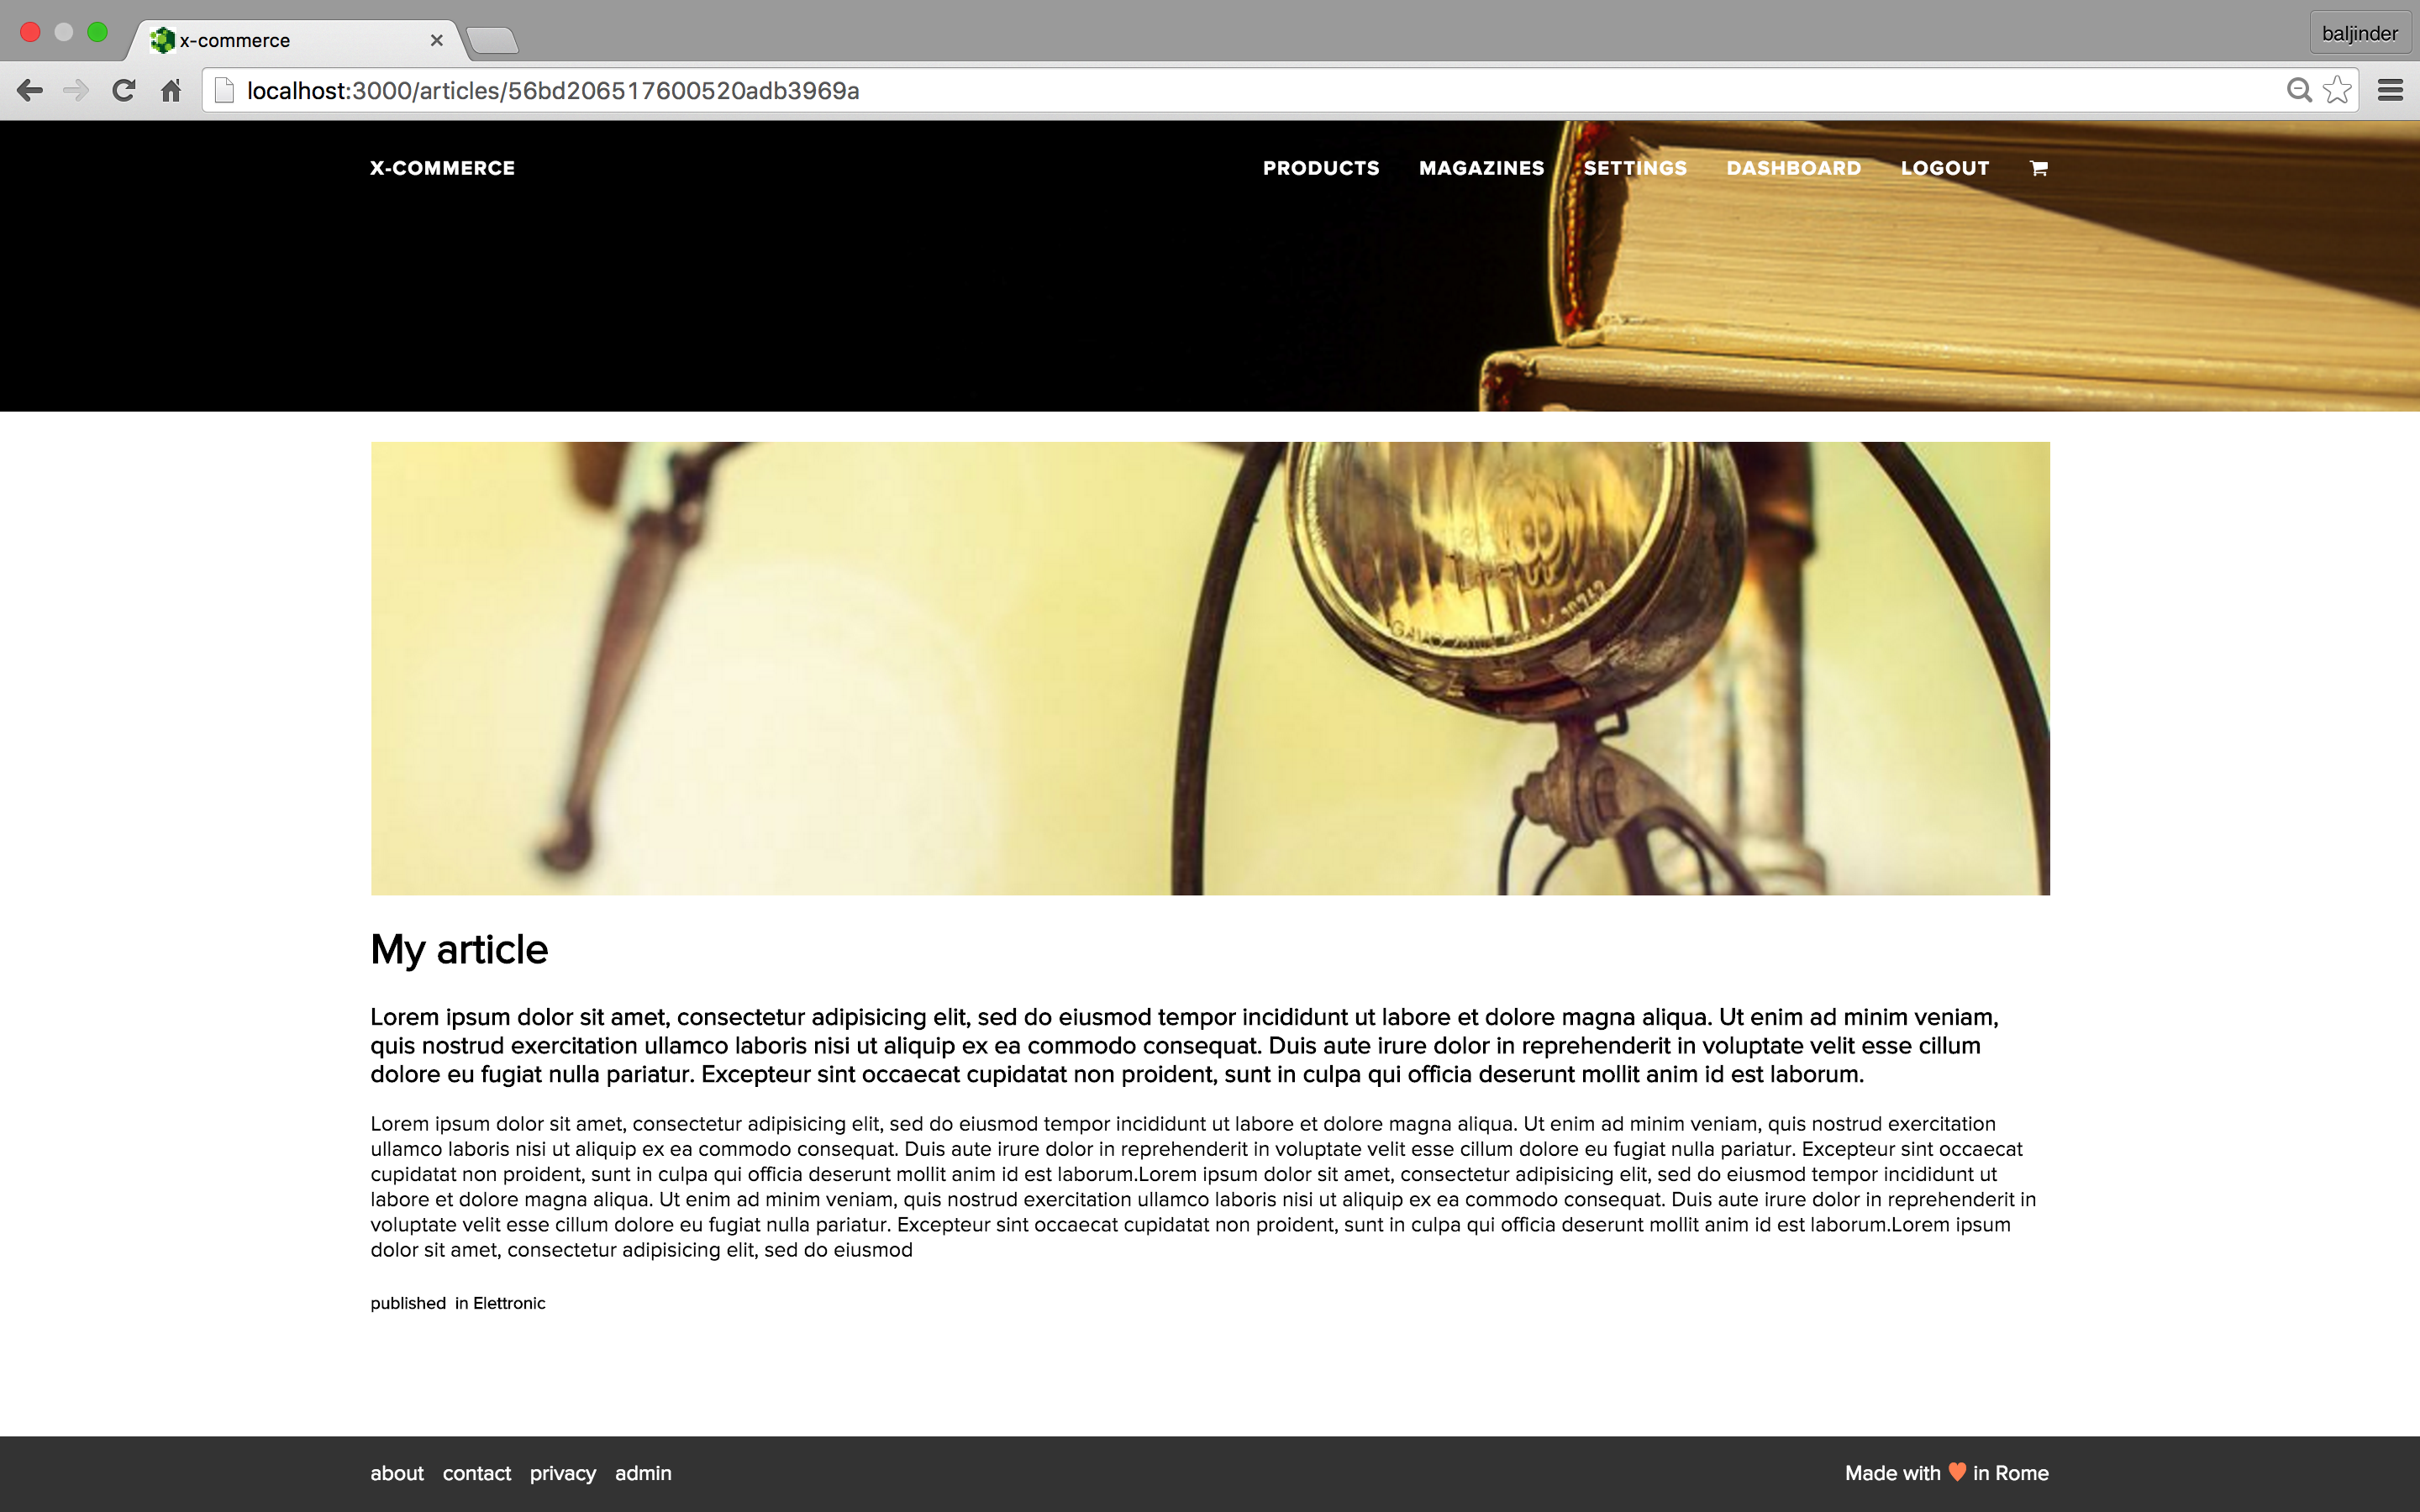
\includegraphics[width=0.84\linewidth]{images/chapter4/page-article-cli.png}\hfill
\caption[Article page on the client-side]{Article page on the client-side}
\label{fig:page_article_cli}
\end{figure}

